% Presentazione Web Services ed ESB - Versione Arricchita
% Autore: Prof. Fedeli Massimo
\documentclass{beamer}
\usetheme{Madrid}
\usecolortheme{default}
\usepackage[utf8]{inputenc}
\usepackage{graphicx}
\usepackage{tikz}
\usetikzlibrary{arrows.meta,shapes.geometric,positioning,shadows,calc,decorations.pathreplacing,fit}
\usepackage{hyperref}
\usepackage{listings}
\usepackage{xcolor}

% Configurazione listing per XML
\lstdefinelanguage{XML}{
	basicstyle=\ttfamily\footnotesize,
	morestring=[b]",
	morestring=[s]{>}{<},
	morecomment=[s]{<?}{?>},
	stringstyle=\color{blue},
	identifierstyle=\color{red},
	keywordstyle=\color{orange},
	commentstyle=\color{green!50!black}
}

\title{Web Services e Enterprise Service Bus}
\subtitle{Architetture di Integrazione per Sistemi Distribuiti}
\author{Prof. Fedeli Massimo}
\institute{IIS Fermi Sacconi Ceci - Ascoli Piceno}
\date{}

\begin{document}
	
	% Titolo
	\begin{frame}
		\titlepage
	\end{frame}
	

	
	\section{Introduzione}
	
	% 1
	\begin{frame}{Obiettivi della presentazione}
		\begin{itemize}
			\item \textbf{Panoramica completa su Web Services}
			\begin{itemize}
				\item SOAP: protocollo di comunicazione XML-based
				\item WSDL: linguaggio di descrizione dei servizi
				\item UDDI: registro per la discovery dei servizi
			\end{itemize}
			\item \textbf{Architetture di integrazione}
			\begin{itemize}
				\item Service-Oriented Architecture (SOA)
				\item Enterprise Application Integration (EAI)
				\item Enterprise Service Bus (ESB)
				\item Java Business Integration (JBI)
			\end{itemize}
			\item \textbf{Pattern e best practices}
			\begin{itemize}
				\item Pattern architetturali e di integrazione
				\item Casi d'uso reali con esempi pratici
			\end{itemize}
		\end{itemize}
	\end{frame}
	
	% 2
	\begin{frame}{Differenza tra Servizi Web e Web Services}
		\begin{columns}
			\column{0.48\textwidth}
			\textbf{Servizi Web (Web Applications)}
			\begin{itemize}
				\item Interfaccia utente (HTML/CSS/JS)
				\item Interazione umana diretta
				\item Browser come client
				\item Output: pagine web visualizzabili
			\end{itemize}
			
			\column{0.48\textwidth}
			\textbf{Web Services}
			\begin{itemize}
				\item Interfaccia programmatica (API)
				\item Integrazione macchina-macchina (M2M)
				\item Applicazioni come client
				\item Output: dati strutturati (XML/JSON)
			\end{itemize}
		\end{columns}
		
		\vspace{0.5cm}
		\begin{alertblock}{Differenza Chiave}
			I Web Services sono progettati per l'integrazione automatizzata tra sistemi software, non per l'interazione umana diretta.
		\end{alertblock}
	\end{frame}
	
	% 3
	\begin{frame}{Evoluzione del Middleware}

		
		\textbf{Motivazione dell'evoluzione:}
		\begin{itemize}
			\item Crescente eterogeneità dei sistemi
			\item Necessità di attraversare firewall
			\item Riduzione del coupling tra componenti
			\item Standard aperti e interoperabili
		\end{itemize}
	\end{frame}
	
	\section{Middleware Tradizionali}
	
	% 4
	\begin{frame}{Modello Client-Server e RPC}
		\begin{columns}
			\column{0.5\textwidth}
			\textbf{Remote Procedure Call (RPC)}
			\begin{itemize}
				\item Chiamata di procedura remota come se fosse locale
				\item Trasparenza della distribuzione
				\item Comunicazione sincrona
				\item Marshalling/unmarshalling parametri
			\end{itemize}
			
			\textbf{Limiti principali:}
			\begin{itemize}
				\item Accoppiamento stretto
				\item Problemi con firewall
				\item Eterogeneità limitata
				\item Gestione errori di rete complessa
			\end{itemize}
			
			\column{0.45\textwidth}
			\begin{center}
				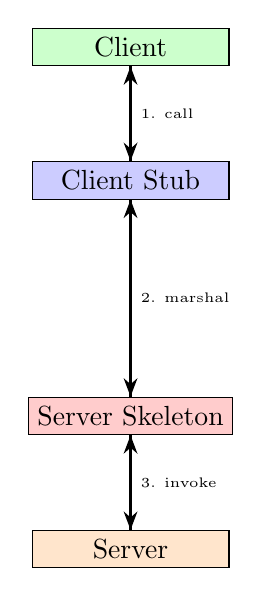
\begin{tikzpicture}[node distance=1.2cm]
					\node[draw,rectangle,fill=green!20,minimum width=2.5cm] (client) {Client};
					\node[draw,rectangle,fill=blue!20,below=of client,minimum width=2.5cm] (stub) {Client Stub};
					\node[draw,rectangle,fill=red!20,below=2.5cm of stub,minimum width=2.5cm] (skel) {Server Skeleton};
					\node[draw,rectangle,fill=orange!20,below=of skel,minimum width=2.5cm] (server) {Server};
					
					\draw[-{Stealth},thick] (client) -- node[right,font=\tiny] {1. call} (stub);
					\draw[-{Stealth},thick] (stub) -- node[right,font=\tiny] {2. marshal} (skel);
					\draw[-{Stealth},thick] (skel) -- node[right,font=\tiny] {3. invoke} (server);
					\draw[-{Stealth},thick,dashed] (server) -- (skel);
					\draw[-{Stealth},thick,dashed] (skel) -- (stub);
					\draw[-{Stealth},thick,dashed] (stub) -- (client);
				\end{tikzpicture}
			\end{center}
		\end{columns}
	\end{frame}
	
	% 5
	\begin{frame}{CORBA: elementi essenziali}
		\textbf{Common Object Request Broker Architecture}
		
		\begin{block}{Componenti principali}
			\begin{itemize}
				\item \textbf{ORB (Object Request Broker)}: middleware per comunicazione oggetti distribuiti
				\item \textbf{IDL (Interface Definition Language)}: linguaggio neutro per definire interfacce
				\item \textbf{Stubs e Skeletons}: proxy client-side e server-side
				\item \textbf{IIOP (Inter-ORB Protocol)}: protocollo di comunicazione tra ORB
			\end{itemize}
		\end{block}
		
		\textbf{Vantaggi:}
		\begin{itemize}
			\item Interoperabilità multi-linguaggio (Java, C++, Python, etc.)
			\item Location transparency
			\item Object-oriented
		\end{itemize}
		
		\textbf{Svantaggi:}
		\begin{itemize}
			\item Complessità di configurazione e deployment
			\item Problemi con firewall (porte dinamiche)
			\item Scarsa adozione oltre l'ambito enterprise
		\end{itemize}
	\end{frame}
	
	% 6
	\begin{frame}{COM/DCOM (.NET)}
		\textbf{Component Object Model / Distributed COM}
		
		\begin{columns}
			\column{0.55\textwidth}
			\textbf{Caratteristiche:}
			\begin{itemize}
				\item Tecnologia Microsoft proprietaria
				\item Integrazione nativa con Windows
				\item Registrazione componenti nel Registry
				\item DCOM per distribuzione su rete
				\item Active Directory per discovery
			\end{itemize}
			
			\textbf{Limitazioni:}
			\begin{itemize}
				\item Piattaforma-dipendente (Windows)
				\item Complessità di configurazione DCOM
				\item Problemi di sicurezza
				\item Difficoltà attraversamento firewall
			\end{itemize}
			
			\column{0.4\textwidth}
			\begin{center}
				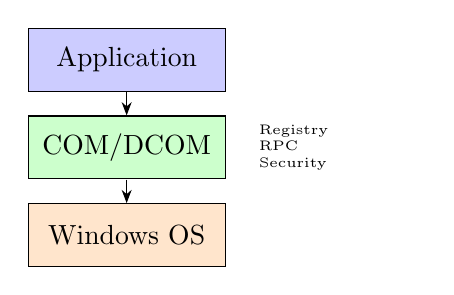
\begin{tikzpicture}[scale=0.8]
					\node[draw,rectangle,fill=blue!20,minimum width=2.5cm,minimum height=0.8cm] (app) {Application};
					\node[draw,rectangle,fill=green!20,below=0.3cm of app,minimum width=2.5cm,minimum height=0.8cm] (com) {COM/DCOM};
					\node[draw,rectangle,fill=orange!20,below=0.3cm of com,minimum width=2.5cm,minimum height=0.8cm] (win) {Windows OS};
										\draw[-{Stealth}] (app) -- (com);
					\draw[-{Stealth}] (com) -- (win);
										\node[right=0.3cm of com,text width=2cm,font=\tiny] {Registry\\RPC\\Security};
				\end{tikzpicture}
			\end{center}
		\end{columns}
		
		\vspace{0.3cm}
		\textbf{Evoluzione:} COM $\rightarrow$ DCOM $\rightarrow$ COM+ $\rightarrow$ .NET Remoting $\rightarrow$ WCF
	\end{frame}
	
	% 7
	\begin{frame}{Sistemi Middleware: confronto rapido}
		\begin{table}
			\tiny
			\begin{tabular}{|l|c|c|c|}
				\hline
				\textbf{Caratteristica} & \textbf{CORBA} & \textbf{DCOM} & \textbf{Web Services} \\
				\hline
				\textbf{Linguaggi} & Multi-linguaggio & Windows-centric & Multi-linguaggio \\
				\hline
				\textbf{Piattaforme} & Multi-piattaforma & Windows & Multi-piattaforma \\
				\hline
				\textbf{Coupling} & Stretto & Stretto & Loose \\
				\hline
				\textbf{Firewall} & Problematico & Problematico & Friendly (HTTP) \\
				\hline
				\textbf{Protocollo} & IIOP & DCOM RPC & SOAP/HTTP \\
				\hline
				\textbf{Discovery} & Naming Service & Active Directory & UDDI/WSIL \\
				\hline
				\textbf{Standard} & OMG & Microsoft & W3C/OASIS \\
				\hline
				\textbf{Complessità} & Alta & Media & Media-Bassa \\
				\hline
				\textbf{Formato dati} & Binario (CDR) & Binario & XML (testuale) \\
				\hline
				\textbf{Performance} & Eccellente & Buona & Media \\
				\hline
			\end{tabular}
		\end{table}
		
		\vspace{0.3cm}
		\begin{alertblock}{Conclusione}
			I Web Services hanno vinto per: \textbf{standard aperti}, \textbf{firewall-friendly}, \textbf{loose coupling} e \textbf{interoperabilità}.
		\end{alertblock}
	\end{frame}
	
	\section{XML e Standard Web Services}
	
	% 8
	\begin{frame}[fragile]{XML come metalinguaggio}
		\textbf{eXtensible Markup Language}
		
		\begin{columns}
			\column{0.5\textwidth}
			\textbf{Caratteristiche:}
			\begin{itemize}
				\item Metalinguaggio per dati strutturati
				\item Self-describing (tag personalizzati)
				\item Human-readable e machine-parseable
				\item Validazione tramite DTD o XSD
				\item Separazione contenuto/presentazione
			\end{itemize}
			
			\textbf{Ruolo nei Web Services:}
			\begin{itemize}
				\item Serializzazione dati
				\item Definizione interfacce (WSDL)
				\item Messaggi SOAP
				\item Configurazione servizi
			\end{itemize}
			
			\column{0.45\textwidth}
			\begin{lstlisting}[language=XML,basicstyle=\ttfamily\tiny]
				<?xml version="1.0"?>
				<libro>
				<titolo>Web Services</titolo>
				<autore>
				<nome>Mario</nome>
				<cognome>Rossi</cognome>
				</autore>
				<anno>2024</anno>
				<prezzo valuta="EUR">
				45.50
				</prezzo>
				</libro>
			\end{lstlisting}
			
			\vspace{0.2cm}
			\textbf{Validazione XSD:}
			\begin{itemize}
				\item Tipi di dati
				\item Struttura documenti
				\item Vincoli di integrità
			\end{itemize}
		\end{columns}
	\end{frame}
	
	% 9
	\begin{frame}{SOAP: panoramica}
		\textbf{Simple Object Access Protocol}
		
		\begin{block}{Definizione}
			Protocollo XML-based per lo scambio di messaggi strutturati in ambienti decentralizzati e distribuiti. Può essere trasportato su HTTP, SMTP, TCP, JMS.
		\end{block}
		
		\textbf{Caratteristiche principali:}
		\begin{itemize}
			\item \textbf{Stateless}: ogni richiesta è indipendente
			\item \textbf{Estensibile}: header personalizzabili per metadati
			\item \textbf{Neutrale}: indipendente da linguaggio e piattaforma
			\item \textbf{Standard}: specifiche W3C ben definite
		\end{itemize}
		
		\textbf{Struttura del messaggio:}
		\begin{itemize}
			\item \textbf{Envelope}: container root del messaggio
			\item \textbf{Header}: informazioni di controllo (opzionale)
			\item \textbf{Body}: payload effettivo del messaggio
			\item \textbf{Fault}: gestione errori e eccezioni
		\end{itemize}
	\end{frame}
	
	% 10
	\begin{frame}{Schema: SOAP Envelope}
		\begin{center}
			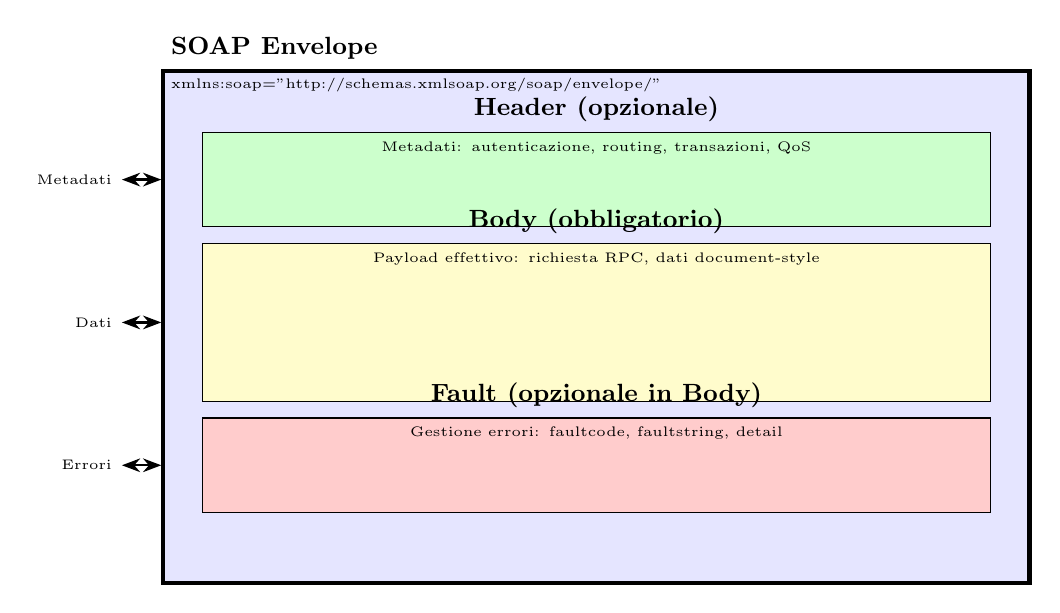
\begin{tikzpicture}[node distance=0mm, every node/.style={font=\small}]
				% Envelope esterno
				\node[draw,rectangle,minimum width=11cm,minimum height=6.5cm,fill=blue!10,line width=1.5pt] (env) {};
				\node[above right] at (env.north west) {\textbf{SOAP Envelope}};
				\node[below right,font=\tiny] at (env.north west) {xmlns:soap="http://schemas.xmlsoap.org/soap/envelope/"};
				
				% Header
				\node[draw,rectangle,below=8mm of env.north,minimum width=10cm,minimum height=1.2cm,fill=green!20] (hdr) {};
				\node[above] at (hdr.north) {\textbf{Header (opzionale)}};
				\node[below,font=\tiny,text width=9cm,align=center] at (hdr.north) {
					Metadati: autenticazione, routing, transazioni, QoS
				};
				
				% Body
				\node[draw,rectangle,below=2mm of hdr,minimum width=10cm,minimum height=2cm,fill=yellow!20] (body) {};
				\node[above] at (body.north) {\textbf{Body (obbligatorio)}};
				\node[below,font=\tiny,text width=9cm,align=center] at (body.north) {
					Payload effettivo: richiesta RPC, dati document-style
				};
				
				% Fault
				\node[draw,rectangle,below=2mm of body,minimum width=10cm,minimum height=1.2cm,fill=red!20] (fault) {};
				\node[above] at (fault.north) {\textbf{Fault (opzionale in Body)}};
				\node[below,font=\tiny,text width=9cm,align=center] at (fault.north) {
					Gestione errori: faultcode, faultstring, detail
				};
				
				% Frecce laterali
				\draw[{Stealth}-{Stealth},thick] (env.west |- hdr) -- ++(-0.5,0) node[left,font=\tiny] {Metadati};
				\draw[{Stealth}-{Stealth},thick] (env.west |- body) -- ++(-0.5,0) node[left,font=\tiny] {Dati};
				\draw[{Stealth}-{Stealth},thick] (env.west |- fault) -- ++(-0.5,0) node[left,font=\tiny] {Errori};
			\end{tikzpicture}
		\end{center}
	\end{frame}
	
	% 11
	\begin{frame}[fragile]{SOAP: esempio di request}
		\textbf{Richiesta GetLastTradePrice per un'azione}
		
		\begin{lstlisting}[language=XML,basicstyle=\ttfamily\tiny]
			<?xml version="1.0"?>
			<soap:Envelope 
			xmlns:soap="http://schemas.xmlsoap.org/soap/envelope/"
			xmlns:m="http://www.stock.org/stock">
			
			<soap:Header>
			<m:Authentication>
			<m:Username>user123</m:Username>
			<m:Password>pass456</m:Password>
			</m:Authentication>
			</soap:Header>
			
			<soap:Body>
			<m:GetLastTradePrice>
			<m:StockSymbol>AAPL</m:StockSymbol>
			</m:GetLastTradePrice>
			</soap:Body>
			
			</soap:Envelope>
		\end{lstlisting}
		
		\textbf{Nota:} La richiesta viene inviata via HTTP POST all'endpoint del servizio.
	\end{frame}
	
	% 12
	\begin{frame}{SOAP: namespace e binding}
		\textbf{Namespace SOAP standard:}
		\begin{itemize}
			\item \texttt{http://schemas.xmlsoap.org/soap/envelope/}
			\item \texttt{http://schemas.xmlsoap.org/soap/encoding/}
		\end{itemize}
		
		\textbf{Encoding Style:}
		\begin{itemize}
			\item \textbf{SOAP Encoding}: regole SOAP per serializzazione
			\item \textbf{Literal}: rispetta esattamente lo schema XSD
		\end{itemize}
		
		\textbf{HTTP Binding:}
		\begin{table}
			\small
			\begin{tabular}{ll}
				\textbf{Header} & \textbf{Valore} \\
				\hline
				Method & POST (tipicamente) \\
				Content-Type & text/xml; charset=utf-8 \\
				SOAPAction & "URI-azione" o "" \\
				Content-Length & lunghezza body \\
			\end{tabular}
		\end{table}
		
		\textbf{SOAPAction header:}
		\begin{itemize}
			\item Indica l'intent della richiesta
			\item Utile per routing e firewall
			\item Può essere stringa vuota ""
		\end{itemize}
	\end{frame}
	
	% 13
	\begin{frame}{Stili di Interazione SOAP}
		\begin{columns}
			\column{0.48\textwidth}
			\textbf{Document-Style}
			\begin{itemize}
				\item Scambio di documenti XML
				\item Asincrono (fire-and-forget)
				\item One-way o notification
				\item Loose coupling
				\item Validazione tramite XSD
			\end{itemize}
			
			\textbf{Uso tipico:}
			\begin{itemize}
				\item Messaggistica asincrona
				\item Event notification
				\item Batch processing
			\end{itemize}
			
			\column{0.48\textwidth}
			\textbf{RPC-Style}
			\begin{itemize}
				\item Chiamata procedura remota
				\item Sincrono (request-response)
				\item Parametri e valori di ritorno
				\item Tight coupling
				\item Encoding SOAP tipico
			\end{itemize}
			
			\textbf{Uso tipico:}
			\begin{itemize}
				\item Query database
				\item Calcoli real-time
				\item Transazioni immediate
			\end{itemize}
		\end{columns}
		
		\vspace{0.5cm}
		\begin{block}{Best Practice}
			\textbf{Document/Literal Wrapped} è lo stile raccomandato: combina validazione XSD con semplicità RPC.
		\end{block}
	\end{frame}
	
	% 14
	\begin{frame}[fragile]{SOAP Fault: gestione errori}
		\textbf{Struttura del Fault element}
		
		\begin{lstlisting}[language=XML,basicstyle=\ttfamily\tiny]
			<soap:Fault>
			<faultcode>soap:Client</faultcode>
			<faultstring>Invalid Stock Symbol</faultstring>
			<faultactor>http://www.stock.org/stockquote</faultactor>
			<detail>
			<e:StockError xmlns:e="http://www.stock.org/errors">
			<e:ErrorCode>1001</e:ErrorCode>
			<e:Message>Symbol XXXX not found in database</e:Message>
			</e:StockError>
			</detail>
			</soap:Fault>
		\end{lstlisting}
		
		\textbf{Fault codes standard:}
		\begin{itemize}
			\item \textbf{VersionMismatch}: versione SOAP non supportata
			\item \textbf{MustUnderstand}: header obbligatorio non compreso
			\item \textbf{Client}: errore nella richiesta del client
			\item \textbf{Server}: errore nell'elaborazione server-side
		\end{itemize}
		
		\textbf{Strategie di gestione:} retry, fallback, logging, alert
	\end{frame}
	
	\section{WSDL e Discovery}
	
	% 15
	\begin{frame}{WSDL: concetti chiave}
		\textbf{Web Services Description Language}
		
		\begin{block}{Scopo}
			Linguaggio XML per descrivere in modo formale e machine-readable le interfacce dei Web Services: operazioni, parametri, tipi di dati, binding e endpoint.
		\end{block}
		
		\textbf{Struttura a due livelli:}
		
		\begin{columns}
			\column{0.48\textwidth}
			\textbf{Parte Astratta}
			\begin{itemize}
				\item \textbf{Types}: schemi XSD per tipi di dati
				\item \textbf{Messages}: definizione messaggi
				\item \textbf{Operations}: operazioni disponibili
				\item \textbf{PortType/Interface}: raggruppamento operazioni
			\end{itemize}
			\textit{Riusabile, indipendente dal protocollo}
			
			\column{0.48\textwidth}
			\textbf{Parte Concreta}
			\begin{itemize}
				\item \textbf{Binding}: protocollo e formato (SOAP/HTTP)
				\item \textbf{Service}: endpoint URL reale
				\item \textbf{Port}: combinazione binding+indirizzo
			\end{itemize}
			\textit{Specifica dell'implementazione}
		\end{columns}
		
		\vspace{0.3cm}
		\textbf{Versioni:} WSDL 1.1 (ampiamente usato) e WSDL 2.0 (raccomandazione W3C)
	\end{frame}
	
	% 16
%	\begin{frame}{Schema: architettura WSDL}
%		\begin{center}
%			\begin{tikzpicture}[
%				node distance=1.5cm,
%				box/.style={draw,rectangle,minimum width=2.5cm,minimum height=0.8cm,rounded corners,font=\small},
%				abstract/.style={fill=blue!20},
%				concrete/.style={fill=orange!20}
%				]
%				
%				% Parte astratta
%				\node[box,abstract] (types) {Types\\(XSD)};
%				\node[box,abstract,right=of types] (message) {Message\\(parts)};
%				\node[box,abstract,right=of message] (operation) {Operation\\(I/O)};
%				\node[box,abstract,right=of operation] (porttype) {PortType\\(Interface)};
%				
%				% Parte concreta
%				\node[box,concrete,below=2cm of porttype] (binding) {Binding\\(SOAP/HTTP)};
%				\node[box,concrete,below=of binding] (port) {Port\\(Endpoint)};
%				\node[box,concrete,below=of port] (service) {Service\\(Collection)};
%				
%				% Connessioni parte astratta
%				\draw[-{Stealth},thick] (types) -- (message) node[midway,above,font=\tiny] {usa};
%				\draw[-{Stealth},thick] (message) -- (operation) node[midway,above,font=\tiny] {compone};
%				\draw[-{Stealth},thick] (operation) -- (porttype) node[midway,above,font=\tiny] {raggruppa};
%				
%				% Connessioni parte concreta
%				\draw[-{Stealth},thick] (porttype) -- (binding) node[midway,right,font=\tiny] {implementa};
%				\draw[-{Stealth},thick] (binding) -- (port) node[midway,right,font=\tiny] {specifica};
%				\draw[-{Stealth},thick] (port) -- (service) node[midway,right,font=\tiny] {raggruppa};
%				
%				% Etichette laterali
%				\node[left=0.3cm of types,rotate=90,font=\small,blue] {ASTRATTO};
%				\node[left=0.3cm of binding,rotate=90,font=\small,orange] {CONCRETO};
%				
%				% Linea di separazione
%				\draw[dashed,thick,gray] ($(types.south west)+(-0.5,-0.8)$) -- ($(porttype.south east)+(0.5,-0.8)$);
%				
%			\end{tikzpicture}
%		\end{center}
%	\end{frame}
	
	% 17
	\begin{frame}[fragile]{WSDL: esempio di types e messages}
		\textbf{Definizione Types (XSD Schema)}
		
		\begin{lstlisting}[language=XML,basicstyle=\ttfamily\tiny]
			<types>
			<schema targetNamespace="http://example.com/stockquote"
			xmlns="http://www.w3.org/2001/XMLSchema">
			<element name="GetLastTradePriceRequest">
			<complexType>
			<all>
			<element name="symbol" type="string"/>
			</all>
			</complexType>
			</element>
			<element name="GetLastTradePriceResponse">
			<complexType>
			<all>
			<element name="price" type="float"/>
			</all>
			</complexType>
			</element>
			</schema>
			</types>
		\end{lstlisting}
		
		\begin{lstlisting}[language=XML,basicstyle=\ttfamily\tiny]
			<message name="GetLastTradePriceInput">
			<part name="body" element="tns:GetLastTradePriceRequest"/>
			</message>
			<message name="GetLastTradePriceOutput">
			<part name="body" element="tns:GetLastTradePriceResponse"/>
			</message>
		\end{lstlisting}
	\end{frame}
	
	% 18
	\begin{frame}[fragile]{WSDL: binding e endpoint}
		\textbf{Binding: collega PortType a protocollo concreto}
		
		\begin{lstlisting}[language=XML,basicstyle=\ttfamily\tiny]
			<binding name="StockQuoteSoapBinding" type="tns:StockQuotePortType">
			<soap:binding style="document" 
			transport="http://schemas.xmlsoap.org/soap/http"/>
			<operation name="GetLastTradePrice">
			<soap:operation soapAction="http://example.com/GetLastTradePrice"/>
			<input>
			<soap:body use="literal"/>
			</input>
			<output>
			<soap:body use="literal"/>
			</output>
			</operation>
			</binding>
		\end{lstlisting}
		
		\textbf{Service ed Endpoint}
		\begin{lstlisting}[language=XML,basicstyle=\ttfamily\tiny]
			<service name="StockQuoteService">
			<port name="StockQuotePort" binding="tns:StockQuoteSoapBinding">
			<soap:address location="http://example.com/stockquote"/>
			</port>
			</service>
		\end{lstlisting}
	\end{frame}
	
	% 19
	\begin{frame}{Uso pratico del WSDL}
		\textbf{Workflow di utilizzo:}
		
		\begin{enumerate}
			\item \textbf{Pubblicazione}: il provider pubblica il WSDL
			\item \textbf{Discovery}: il consumer trova il WSDL (UDDI, URL, registry)
			\item \textbf{Generazione stub}: tool automatici creano proxy client
			\begin{itemize}
				\item Java: wsimport, Axis, CXF
				\item .NET: wsdl.exe, svcutil.exe
				\item Python: suds, zeep
			\end{itemize}
			\item \textbf{Invocazione}: il client usa lo stub come oggetto locale
			\item \textbf{Validazione}: verifica automatica parametri contro schema
		\end{enumerate}
		
		\vspace{0.3cm}
		\textbf{Vantaggi:}
		\begin{itemize}
			\item Contract-first development
			\item Type-safety compile-time
			\item Documentazione machine-readable
			\item Interoperabilità garantita
		\end{itemize}
	\end{frame}
	
	% 20
	\begin{frame}{UDDI: panoramica}
		\textbf{Universal Description, Discovery and Integration}
		
		\begin{block}{Motivazione}
			Registry distribuito per pubblicare e scoprire Web Services. Concetto analogo alle "Pagine Gialle" per i servizi web.
		\end{block}
		
		\textbf{Tre componenti principali:}
		\begin{itemize}
			\item \textbf{White Pages}: informazioni di contatto business (nome, indirizzo, etc.)
			\item \textbf{Yellow Pages}: classificazione per categoria industriale/geografica
			\item \textbf{Green Pages}: informazioni tecniche sui servizi (WSDL, binding)
		\end{itemize}
		
		\textbf{Entità del modello dati:}
		\begin{itemize}
			\item \textbf{businessEntity}: organizzazione che pubblica servizi
			\item \textbf{businessService}: descrizione logica del servizio
			\item \textbf{bindingTemplate}: dettagli tecnici accesso (URL, protocollo)
			\item \textbf{tModel (technical model)}: metadati e specifiche tecniche
		\end{itemize}
	\end{frame}
	
	% 21
	\begin{frame}{Schema: modello UDDI}
		\begin{center}
			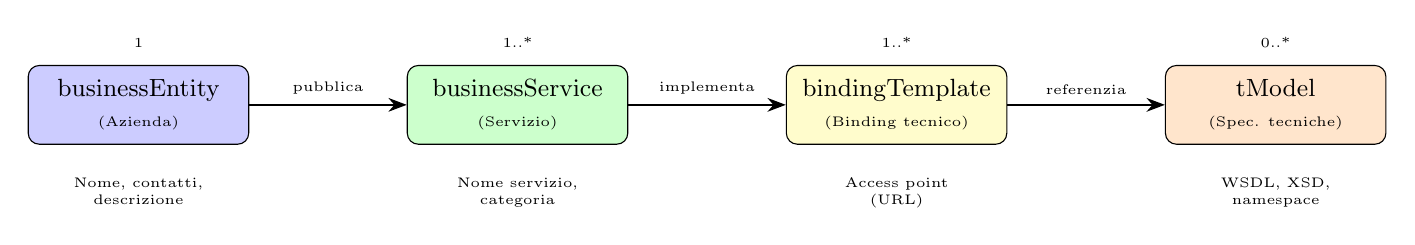
\begin{tikzpicture}[
				node distance=2cm,
				box/.style={draw,rectangle,minimum width=2.8cm,minimum height=1cm,rounded corners,font=\small,align=center},
				level1/.style={fill=blue!20},
				level2/.style={fill=green!20},
				level3/.style={fill=yellow!20},
				level4/.style={fill=orange!20}
				]
				
				\node[box,level1] (be) {businessEntity\\{\tiny (Azienda)}};
				\node[box,level2,right=of be] (bs) {businessService\\{\tiny (Servizio)}};
				\node[box,level3,right=of bs] (bt) {bindingTemplate\\{\tiny (Binding tecnico)}};
				\node[box,level4,right=of bt] (tm) {tModel\\{\tiny (Spec. tecniche)}};
				
				\draw[-{Stealth},thick] (be) -- (bs) node[midway,above,font=\tiny] {pubblica};
				\draw[-{Stealth},thick] (bs) -- (bt) node[midway,above,font=\tiny] {implementa};
				\draw[-{Stealth},thick] (bt) -- (tm) node[midway,above,font=\tiny] {referenzia};
				
				% Annotazioni sotto
				\node[below=0.3cm of be,text width=2.5cm,align=center,font=\tiny] {Nome, contatti,\\descrizione};
				\node[below=0.3cm of bs,text width=2.5cm,align=center,font=\tiny] {Nome servizio,\\categoria};
				\node[below=0.3cm of bt,text width=2.5cm,align=center,font=\tiny] {Access point\\(URL)};
				\node[below=0.3cm of tm,text width=2.5cm,align=center,font=\tiny] {WSDL, XSD,\\namespace};
				
				% Cardinalità
				\node[above=0.1cm of be,font=\tiny] {1};
				\node[above=0.1cm of bs,font=\tiny] {1..*};
				\node[above=0.1cm of bt,font=\tiny] {1..*};
				\node[above=0.1cm of tm,font=\tiny] {0..*};
				
			\end{tikzpicture}
		\end{center}
		
		\vspace{0.3cm}
		\textbf{Operazioni UDDI:}
		\begin{itemize}
			\item \textbf{Publish API}: registrazione e aggiornamento servizi
			\item \textbf{Inquiry API}: ricerca e recupero informazioni
		\end{itemize}
	\end{frame}
	
	% 22
	\begin{frame}{UDDI: White/Yellow/Green Pages}
		\begin{center}
			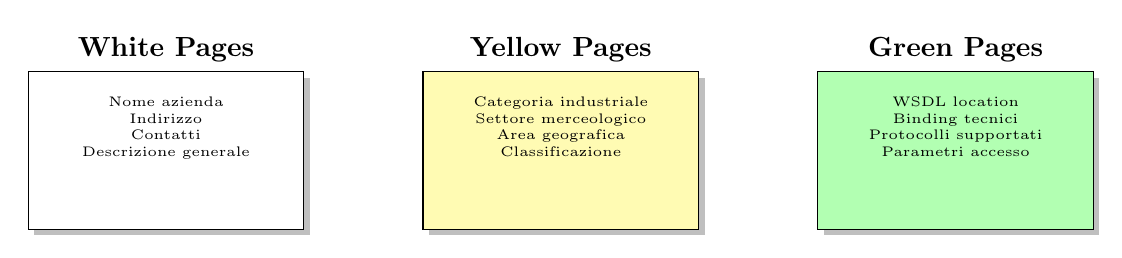
\begin{tikzpicture}[node distance=1.5cm]
				
				% White Pages
				\node[draw,rectangle,fill=white,minimum width=3.5cm,minimum height=2cm,drop shadow] (white) {};
				\node[above] at (white.north) {\textbf{White Pages}};
				\node[below=0.2cm of white.north,text width=3cm,align=center,font=\tiny] {
					Nome azienda\\
					Indirizzo\\
					Contatti\\
					Descrizione generale
				};
				
				% Yellow Pages
				\node[draw,rectangle,fill=yellow!30,minimum width=3.5cm,minimum height=2cm,drop shadow,right=of white] (yellow) {};
				\node[above] at (yellow.north) {\textbf{Yellow Pages}};
				\node[below=0.2cm of yellow.north,text width=3cm,align=center,font=\tiny] {
					Categoria industriale\\
					Settore merceologico\\
					Area geografica\\
					Classificazione
				};
				
				% Green Pages
				\node[draw,rectangle,fill=green!30,minimum width=3.5cm,minimum height=2cm,drop shadow,right=of yellow] (green) {};
				\node[above] at (green.north) {\textbf{Green Pages}};
				\node[below=0.2cm of green.north,text width=3cm,align=center,font=\tiny] {
					WSDL location\\
					Binding tecnici\\
					Protocolli supportati\\
					Parametri accesso
				};
				
			\end{tikzpicture}
		\end{center}
		
		\vspace{0.5cm}
		\textbf{Esempio ricerca:}
		\begin{enumerate}
			\item Cerco in Yellow Pages: "servizi finanziari" + "Roma"
			\item Ottengo lista aziende (White Pages)
			\item Per ogni azienda, accedo ai dettagli tecnici (Green Pages)
			\item Download WSDL e generazione stub client
		\end{enumerate}
	\end{frame}
	
	% 23
	\begin{frame}{WSIL: ispezione leggera dei servizi}
		\textbf{Web Services Inspection Language}
		
		\begin{block}{Motivazione}
			Alternativa più semplice e decentralizzata a UDDI. Documento XML statico che elenca i servizi disponibili su un server.
		\end{block}
		
		\textbf{Caratteristiche:}
		\begin{itemize}
			\item File \texttt{inspection.wsil} nella root del web server
			\item Contiene link a WSDL e altri documenti WSIL
			\item Non richiede infrastruttura registry centralizzata
			\item Scoperta gerarchica e distribuita
		\end{itemize}
		
		\textbf{Confronto con UDDI:}
		\begin{table}
			\small
			\begin{tabular}{lcc}
				& \textbf{UDDI} & \textbf{WSIL} \\
				\hline
				Centralizzato & Sì & No \\
				Ricerca & Potente & Limitata \\
				Complessità & Alta & Bassa \\
				Uso tipico & Pubblico & Intranet \\
			\end{tabular}
		\end{table}
		
		\textbf{Situazione attuale:} UDDI pubblici dismessi; WSIL usato in ambito enterprise
	\end{frame}
	
	\section{Performance e Tecnologie Avanzate}
	
	% 24
	\begin{frame}{Performance dei Web Services}
		\textbf{Fattori che impattano le performance:}
		
		\begin{columns}
			\column{0.5\textwidth}
			\textbf{Overhead XML:}
			\begin{itemize}
				\item Parsing e serializzazione
				\item Dimensione messaggi (verbosità)
				\item Validazione schema
			\end{itemize}
			
			\textbf{Overhead HTTP:}
			\begin{itemize}
				\item Latenza connessione TCP
				\item Header HTTP
				\item Nessuna connessione persistente (HTTP/1.0)
			\end{itemize}
			
			\textbf{Overhead SOAP:}
			\begin{itemize}
				\item Envelope wrapping
				\item Namespace processing
				\item Encoding/decoding
			\end{itemize}
			
			\column{0.45\textwidth}
			\textbf{Strategie di ottimizzazione:}
			\begin{enumerate}
				\item \textbf{Caching}: response caching
				\item \textbf{Compressione}: gzip HTTP
				\item \textbf{Batching}: aggregare richieste
				\item \textbf{Binary attachments}: MTOM/XOP
				\item \textbf{Keep-alive}: HTTP/1.1 persistent
				\item \textbf{Asynchronous}: non-blocking I/O
				\item \textbf{Load balancing}: distribuire carico
			\end{enumerate}
		\end{columns}
		
		\vspace{0.3cm}
		\begin{alertblock}{Nota}
			REST/JSON ha generalmente performance migliori per payload piccoli, ma SOAP offre maggiori funzionalità enterprise (transazioni, sicurezza, etc.)
		\end{alertblock}
	\end{frame}
	
	% 25
	\begin{frame}{Ciclo di adozione tecnologica}
		\textbf{Gartner Hype Cycle}
		
		\begin{center}
			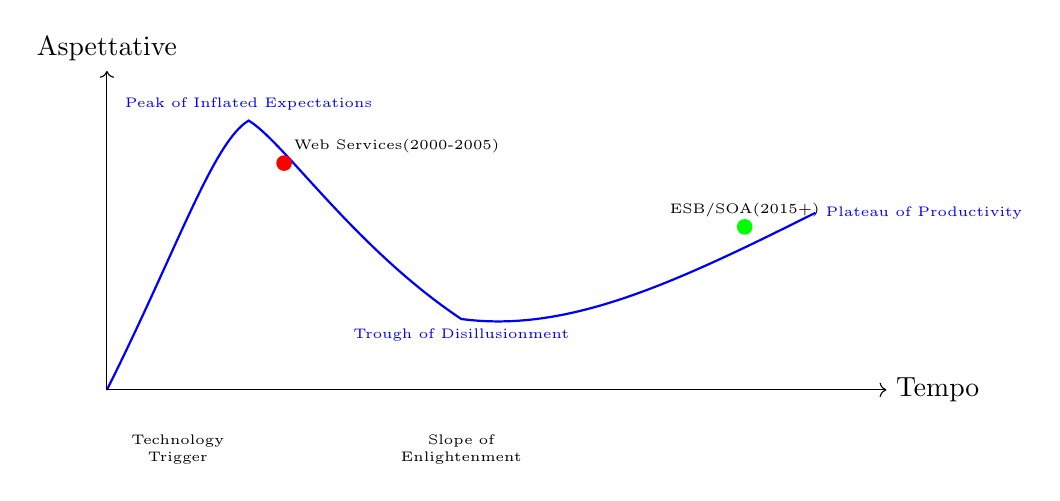
\begin{tikzpicture}[scale=0.9]
				% Curva hype cycle
				\draw[thick,blue] (0,0) 
				.. controls (1,2) and (1.5,3.5) .. (2,3.8) 
				node[above,font=\tiny] {Peak of Inflated Expectations}
				.. controls (2.5,3.5) and (3.5,2) .. (5,1) 
				node[below,font=\tiny] {Trough of Disillusionment}
				.. controls (6.5,0.8) and (8,1.5) .. (10,2.5) 
				node[right,font=\tiny] {Plateau of Productivity};
				
				% Asse
				\draw[->] (0,0) -- (11,0) node[right] {Tempo};
				\draw[->] (0,0) -- (0,4.5) node[above] {Aspettative};
				
				% Posizionamento tecnologie (indicativo)
				\node[circle,fill=red,inner sep=2pt] at (2.5,3.2) {};
				\node[above right,font=\tiny] at (2.5,3.2) {Web Services\\(2000-2005)};
				
				\node[circle,fill=green,inner sep=2pt] at (9,2.3) {};
				\node[above,font=\tiny] at (9,2.3) {ESB/SOA\\(2015+)};
				
				% Fasi
				\node[below,font=\tiny,text width=2cm,align=center] at (1,-0.5) {Technology\\Trigger};
				\node[below,font=\tiny,text width=2cm,align=center] at (5,-0.5) {Slope of\\Enlightenment};
				
			\end{tikzpicture}
		\end{center}
		
		\textbf{Evoluzione:}
		\begin{itemize}
			\item \textbf{2000-2005}: hype massimo su Web Services
			\item \textbf{2005-2010}: delusione, complessità, REST emerge
			\item \textbf{2010-2015}: maturazione, uso enterprise consolidato
			\item \textbf{2015+}: integrazione con cloud, microservizi, ESB moderni
		\end{itemize}
	\end{frame}
	
	% 26
	\begin{frame}{BPEL4WS: orchestrazione}
		\textbf{Business Process Execution Language for Web Services}
		
		\begin{block}{Definizione}
			Linguaggio XML per orchestrare Web Services in processi di business complessi. Permette di definire flussi di lavoro che coordinano l'invocazione di multipli servizi.
		\end{block}
		
		\textbf{Costrutti principali:}
		\begin{itemize}
			\item \textbf{Sequence}: esecuzione sequenziale di attività
			\item \textbf{Flow}: esecuzione parallela (fork/join)
			\item \textbf{Switch/If}: decisioni condizionali
			\item \textbf{While/RepeatUntil}: cicli iterativi
			\item \textbf{Invoke}: chiamata a Web Service
			\item \textbf{Receive/Reply}: ricezione richieste e invio risposte
			\item \textbf{Assign}: manipolazione variabili
			\item \textbf{Throw/Catch}: gestione eccezioni
		\end{itemize}
		
		\textbf{Caratteristiche:}
		\begin{itemize}
			\item Basato su WSDL per interfacce
			\item Supporto transazioni e compensazioni
			\item Long-running processes
		\end{itemize}
	\end{frame}
	
	% 27
	\begin{frame}{Diagramma: processo BPEL semplificato}
		\begin{center}
			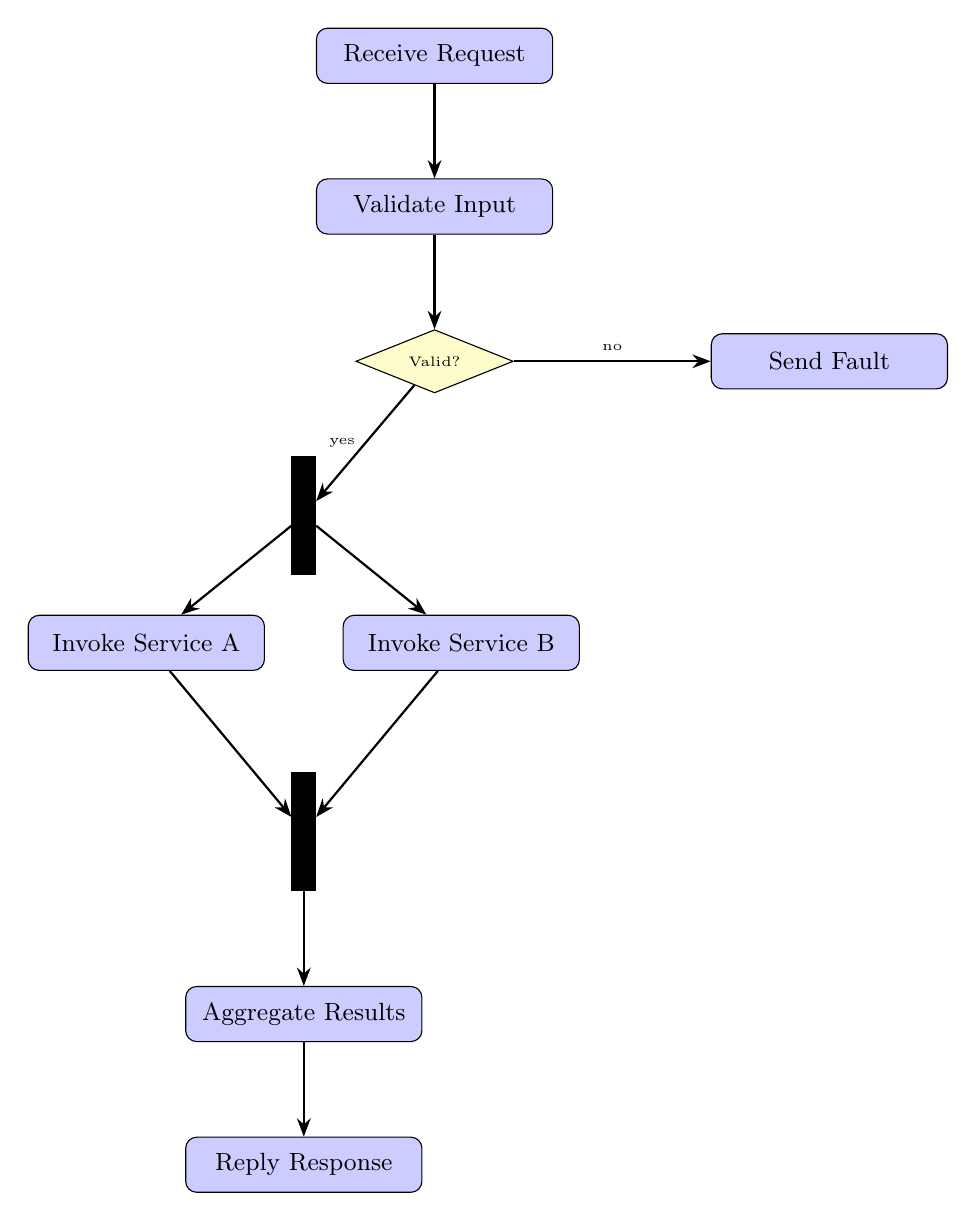
\begin{tikzpicture}[
				node distance=1.2cm,
				activity/.style={draw,rectangle,rounded corners,minimum width=3cm,minimum height=0.7cm,fill=blue!20,font=\small},
				decision/.style={draw,diamond,aspect=2,minimum width=2cm,fill=yellow!20,font=\tiny},
				parallel/.style={draw,rectangle,minimum width=0.3cm,minimum height=1.5cm,fill=black}
				]
				
				\node[activity] (start) {Receive Request};
				\node[activity,below=of start] (validate) {Validate Input};
				\node[decision,below=of validate] (check) {Valid?};
				
				\node[parallel,below left=1cm and 1cm of check] (fork) {};
				\node[activity,below=0.5cm of fork,xshift=-2cm] (serviceA) {Invoke Service A};
				\node[activity,below=0.5cm of fork,xshift=2cm] (serviceB) {Invoke Service B};
				\node[parallel,below=2.5cm of fork] (join) {};
				
				\node[activity,below=of join] (aggregate) {Aggregate Results};
				\node[activity,below=of aggregate] (reply) {Reply Response};
				
				\node[activity,right=2.5cm of check] (error) {Send Fault};
				
				\draw[-{Stealth},thick] (start) -- (validate);
				\draw[-{Stealth},thick] (validate) -- (check);
				\draw[-{Stealth},thick] (check) -- (fork) node[midway,left,font=\tiny] {yes};
				\draw[-{Stealth},thick] (check) -- (error) node[midway,above,font=\tiny] {no};
				\draw[-{Stealth},thick] (fork) -- (serviceA);
				\draw[-{Stealth},thick] (fork) -- (serviceB);
				\draw[-{Stealth},thick] (serviceA) -- (join);
				\draw[-{Stealth},thick] (serviceB) -- (join);
				\draw[-{Stealth},thick] (join) -- (aggregate);
				\draw[-{Stealth},thick] (aggregate) -- (reply);
				
			\end{tikzpicture}
		\end{center}
	\end{frame}
	
	% 28
	\begin{frame}{Orchestrazione vs Coreografia}
		\begin{columns}
			\column{0.48\textwidth}
			\textbf{Orchestrazione}
			\begin{itemize}
				\item \textbf{Controllo centralizzato}
				\item Un orchestratore coordina
				\item Visione globale del processo
				\item BPEL tipicamente
				\item Single point of control
				\item Più facile da monitorare
			\end{itemize}
			
			\begin{center}
				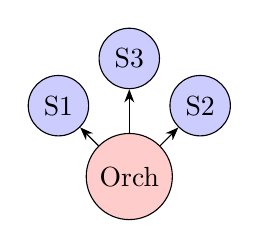
\begin{tikzpicture}[scale=0.6]
					\node[draw,circle,fill=red!20] (orch) at (0,0) {Orch};
					\node[draw,circle,fill=blue!20] (s1) at (-1.5,1.5) {S1};
					\node[draw,circle,fill=blue!20] (s2) at (1.5,1.5) {S2};
					\node[draw,circle,fill=blue!20] (s3) at (0,2.5) {S3};
					\draw[-{Stealth}] (orch) -- (s1);
					\draw[-{Stealth}] (orch) -- (s2);
					\draw[-{Stealth}] (orch) -- (s3);
				\end{tikzpicture}
			\end{center}
			
			\column{0.48\textwidth}
			\textbf{Coreografia}
			\begin{itemize}
				\item \textbf{Coordinamento distribuito}
				\item Ogni servizio sa cosa fare
				\item Peer-to-peer interaction
				\item WS-CDL, event-driven
				\item Maggiore resilienza
				\item Più complesso da debuggare
			\end{itemize}
			
			\begin{center}
				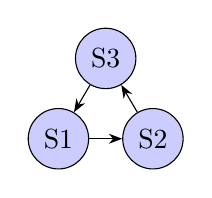
\begin{tikzpicture}[scale=0.6]
					\node[draw,circle,fill=blue!20] (s1) at (0,0) {S1};
					\node[draw,circle,fill=blue!20] (s2) at (2,0) {S2};
					\node[draw,circle,fill=blue!20] (s3) at (1,1.7) {S3};
					\draw[-{Stealth}] (s1) -- (s2);
					\draw[-{Stealth}] (s2) -- (s3);
					\draw[-{Stealth}] (s3) -- (s1);
				\end{tikzpicture}
			\end{center}
		\end{columns}
		
		\vspace{0.5cm}
		\begin{block}{Quando usare}
			\textbf{Orchestrazione}: processi complessi, controllo fine-grained\\
			\textbf{Coreografia}: sistemi decentralizzati, scalabilità, autonomia
		\end{block}
	\end{frame}
	
	% 29
	\begin{frame}{Integrazione: pattern find-bind-invoke}
		\textbf{Il paradigma SOA fondamentale}
		
		\begin{center}
			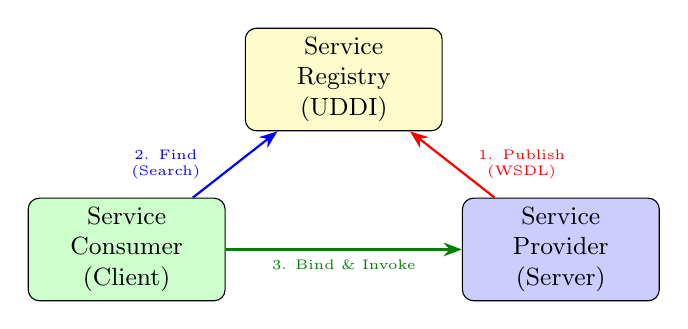
\begin{tikzpicture}[
				node distance=3cm,
				actor/.style={draw,rectangle,rounded corners,minimum width=2.5cm,minimum height=1cm,font=\small,align=center}
				]
				
				\node[actor,fill=green!20] (consumer) {Service\\Consumer\\(Client)};
				\node[actor,fill=blue!20,right=of consumer] (provider) {Service\\Provider\\(Server)};
				\node[actor,fill=yellow!20,above=1.5cm of $(consumer)!0.5!(provider)$] (registry) {Service\\Registry\\(UDDI)};
				
				% Frecce
				\draw[-{Stealth},thick,red] (provider) -- (registry) node[midway,right,font=\tiny,text width=1.5cm,align=center] {1. Publish\\(WSDL)};
				\draw[-{Stealth},thick,blue] (consumer) -- (registry) node[midway,left,font=\tiny,text width=1.5cm,align=center] {2. Find\\(Search)};
				\draw[-{Stealth},thick,green!50!black] (consumer) -- (provider) node[midway,below,font=\tiny] {3. Bind \& Invoke};
				
			\end{tikzpicture}
		\end{center}
		
		\textbf{Fasi dettagliate:}
		\begin{enumerate}
			\item \textbf{Publish}: il provider registra il servizio nel registry con WSDL
			\item \textbf{Find}: il consumer cerca servizi per categoria/nome
			\item \textbf{Bind}: download WSDL e generazione stub/proxy
			\item \textbf{Invoke}: chiamata effettiva al servizio via SOAP
		\end{enumerate}
		
		\textbf{Vantaggi:} loose coupling, discovery dinamico, flessibilità
	\end{frame}
	
	% 30
	\begin{frame}{Gateway e firewall}
		\textbf{Web Services e sicurezza di rete}
		
		\begin{block}{Vantaggio chiave}
			I Web Services usano HTTP/HTTPS (porte 80/443) che attraversano facilmente firewall e proxy aziendali, a differenza di CORBA o DCOM che usano porte dinamiche.
		\end{block}
		
		\begin{center}
			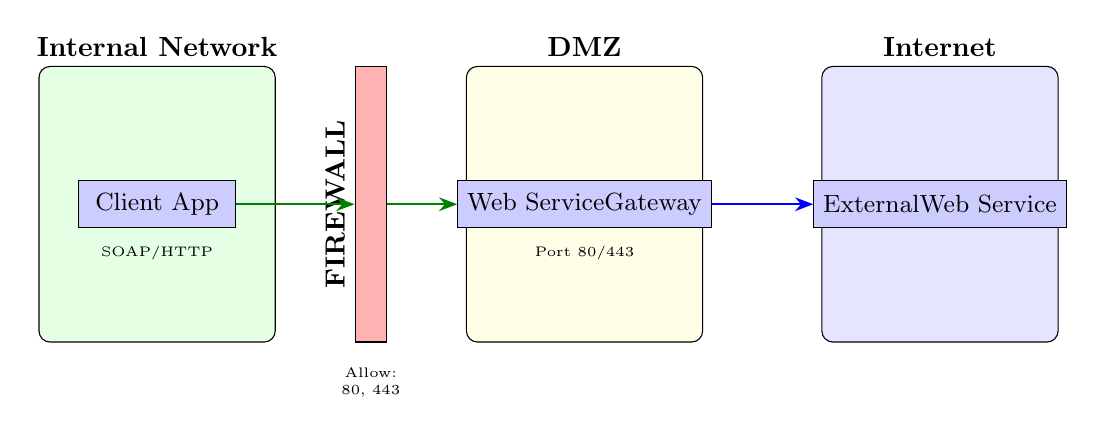
\begin{tikzpicture}[
				node distance=1.5cm,
				zone/.style={draw,rectangle,minimum width=3cm,minimum height=3.5cm,rounded corners},
				server/.style={draw,rectangle,fill=blue!20,minimum width=2cm,minimum height=0.6cm,font=\small}
				]
				
				% Zona interna
				\node[zone,fill=green!10] (internal) {};
				\node[above] at (internal.north) {\textbf{Internal Network}};
				\node[server] (client) at (internal.center) {Client App};
				
				% Firewall
				\node[draw,rectangle,fill=red!30,minimum width=0.4cm,minimum height=3.5cm,right=1cm of internal] (firewall) {};
				\node[above,rotate=90] at (firewall.west) {\textbf{FIREWALL}};
				\node[below=0.2cm of firewall,font=\tiny,text width=2cm,align=center] {Allow:\\80, 443};
				
				% Zona DMZ
				\node[zone,fill=yellow!10,right=1cm of firewall] (dmz) {};
				\node[above] at (dmz.north) {\textbf{DMZ}};
				\node[server] (proxy) at (dmz.center) {Web Service\\Gateway};
				
				% Internet
				\node[zone,fill=blue!10,right=1.5cm of dmz] (internet) {};
				\node[above] at (internet.north) {\textbf{Internet}};
				\node[server] (ws) at (internet.center) {External\\Web Service};
				
				% Connessioni
				\draw[-{Stealth},thick,green!50!black] (client) -- (firewall);
				\draw[-{Stealth},thick,green!50!black] (firewall) -- (proxy);
				\draw[-{Stealth},thick,blue] (proxy) -- (ws);
				
				\node[below=0.1cm of client,font=\tiny] {SOAP/HTTP};
				\node[below=0.1cm of proxy,font=\tiny] {Port 80/443};
				
			\end{tikzpicture}
		\end{center}
		
		\textbf{Componenti:}
		\begin{itemize}
			\item \textbf{Gateway/Proxy}: intermediario in DMZ, filtraggio, logging
			\item \textbf{SSL/TLS}: cifratura end-to-end con HTTPS
		\end{itemize}
	\end{frame}
	
	% 31
	\begin{frame}{Sicurezza nei Web Services}
		\textbf{Livelli di sicurezza}
		
		\begin{enumerate}
			\item \textbf{Transport Level Security}
			\begin{itemize}
				\item HTTPS/TLS: cifratura e autenticazione server
				\item HTTP Basic/Digest Auth
				\item Protegge solo punto-a-punto
			\end{itemize}
			
			\item \textbf{Message Level Security}
			\begin{itemize}
				\item WS-Security: sicurezza end-to-end
				\item XML Signature: integrità e non-ripudio
				\item XML Encryption: confidenzialità
				\item Security tokens: SAML, X.509, Kerberos
			\end{itemize}
		\end{enumerate}
		
		\textbf{Standard WS-Security:}
		\begin{itemize}
			\item \textbf{UsernameToken}: credenziali nell'header SOAP
			\item \textbf{BinarySecurityToken}: certificati X.509
			\item \textbf{SAML Token}: asserzioni di autenticazione/autorizzazione
			\item \textbf{Timestamp}: prevenzione replay attacks
		\end{itemize}
		
		\textbf{Best practices:}
		\begin{itemize}
			\item Sempre HTTPS in produzione
			\item WS-Security per scenari multi-hop
			\item Validazione input per prevenire XML injection
		\end{itemize}
	\end{frame}
	
	% 32
	\begin{frame}{Schema: flusso sicuro con WS-Security}
		\begin{center}
			\begin{tikzpicture}[
				node distance=1.2cm,
				step/.style={draw,rectangle,rounded corners,minimum width=3cm,minimum height=0.7cm,fill=blue!20,font=\small}
				]
				
				\node[draw,circle,fill=green!20,minimum size=1.2cm] (client) {Client};
				\node[step,right=2cm of client] (sign) {1. Sign\\Message};
				\node[step,right=of sign] (encrypt) {2. Encrypt\\Parts};
				\node[step,below=of encrypt] (send) {3. Send SOAP\\+Token};
				\node[step,below=of sign] (decrypt) {5. Decrypt};
				\node[step,left=of decrypt] (verify) {6. Verify\\Signature};
				\node[draw,circle,fill=orange!20,minimum size=1.2cm,left=2cm of verify] (service) {Service};
				
				% Frecce
				\draw[-{Stealth},thick] (client) -- (sign);
				\draw[-{Stealth},thick] (sign) -- (encrypt);
				\draw[-{Stealth},thick] (encrypt) -- (send);
				\draw[-{Stealth},thick] (send) -- (decrypt) node[midway,right,font=\tiny,text width=1.8cm] {4. HTTPS\\Transport};
				\draw[-{Stealth},thick] (decrypt) -- (verify);
				\draw[-{Stealth},thick] (verify) -- (service);
				
				% Annotazioni
				\node[below=0.1cm of sign,font=\tiny,text width=2.5cm,align=center] {XML Signature\\(private key)};
				\node[below=0.1cm of encrypt,font=\tiny,text width=2.5cm,align=center] {XML Encryption\\(public key service)};
				\node[below=0.1cm of verify,font=\tiny,text width=2.5cm,align=center] {Verifica con\\public key client};
				
			\end{tikzpicture}
		\end{center}
		
		\vspace{0.3cm}
		\textbf{Elementi nel messaggio:}
		\begin{itemize}
			\item \textbf{wsse:Security} header con token, signature, encryption references
			\item \textbf{ds:Signature}: firma digitale di parti del messaggio
			\item \textbf{xenc:EncryptedData}: parti cifrate del payload
		\end{itemize}
	\end{frame}
	
	% 33
	\begin{frame}{Estensioni e specifiche correlate}
		\textbf{WS-* Stack: famiglia di specifiche enterprise}
		
		\begin{table}
			\small
			\begin{tabular}{ll}
				\textbf{Specifica} & \textbf{Funzione} \\
				\hline
				WS-Security & Sicurezza messaggi (firma, cifratura, token) \\
				WS-Policy & Dichiarazione requisiti e capability \\
				WS-Addressing & Routing, addressing endpoint-neutral \\
				WS-ReliableMessaging & Garanzia delivery, ordering, deduplication \\
				WS-AtomicTransaction & Transazioni distribuite (2PC) \\
				WS-Coordination & Coordinamento processi distribuiti \\
				WS-BPEL & Orchestrazione processi di business \\
				WS-Discovery & Discovery dinamico servizi su rete \\
				WS-Eventing & Publish/subscribe event notification \\
				WS-Trust & Trust model, token issuance \\
			\end{tabular}
		\end{table}
		
		\vspace{0.3cm}
		\begin{alertblock}{Complessità}
			Lo stack WS-* è molto potente ma anche complesso. In molti scenari REST/JSON è preferito per semplicità, mentre WS-* resta per enterprise mission-critical.
		\end{alertblock}
	\end{frame}
	
	% 34
	\begin{frame}{Composizione e gestione degli errori}
		\textbf{Fault Handling in processi distribuiti}
		
		\begin{block}{Problema}
			In orchestrazioni che coinvolgono multipli servizi, un errore in un punto qualsiasi richiede strategie di ripristino per mantenere coerenza.
		\end{block}
		
		\textbf{Strategie:}
		\begin{enumerate}
			\item \textbf{Retry}: tentativi ripetuti con backoff esponenziale
			\item \textbf{Timeout}: limite temporale per ogni invocazione
			\item \textbf{Fallback}: servizio alternativo se primario fallisce
			\item \textbf{Circuit Breaker}: evitare cascading failures
			\item \textbf{Compensating Transactions}: annullare operazioni già completate
		\end{enumerate}
		
		\textbf{Compensazioni:}
		\begin{itemize}
			\item Ogni attività ha un'azione compensativa inversa
			\item In caso di errore, esecuzione compensazioni in ordine inverso
			\item Esempio: prenotazione volo + hotel
			\begin{itemize}
				\item Successo: volo OK, hotel OK
				\item Fallimento hotel: compensa cancellando volo già prenotato
			\end{itemize}
		\end{itemize}
		
		\textbf{BPEL:} supporta nativamente <compensationHandler> e <faultHandlers>
	\end{frame}
	
	\section{Enterprise Application Integration}
	
	% 35
	\begin{frame}{EAI: approccio tradizionale}
		\textbf{Enterprise Application Integration}
		
		\begin{block}{Definizione}
			Insieme di tecnologie e processi per integrare applicazioni enterprise eterogenee (ERP, CRM, SCM, legacy systems) per condividere dati e processi.
		\end{block}
		
		\textbf{Approcci storici:}
		\begin{itemize}
			\item \textbf{Point-to-Point}: connessioni dirette tra applicazioni
			\begin{itemize}
				\item Pro: semplice inizialmente
				\item Contro: O(n²) connessioni, manutenzione impossibile
			\end{itemize}
			
			\item \textbf{Hub-and-Spoke}: broker centralizzato
			\begin{itemize}
				\item Pro: centralizzazione, O(n) connessioni
				\item Contro: single point of failure, bottleneck
			\end{itemize}
			
			\item \textbf{Enterprise Service Bus (ESB)}: bus distribuito
			\begin{itemize}
				\item Pro: scalabilità, resilienza, standard
				\item Contro: complessità configurazione
			\end{itemize}
		\end{itemize}
		
		\textbf{Tecniche EAI:}
		\begin{itemize}
			\item \textbf{ETL}: Extract, Transform, Load per batch integration
			\item \textbf{Messaging}: code asincrone per eventi real-time
		\end{itemize}
	\end{frame}
	
	% 36
	\begin{frame}{Schema: Hub-and-Spoke}
		\begin{center}
			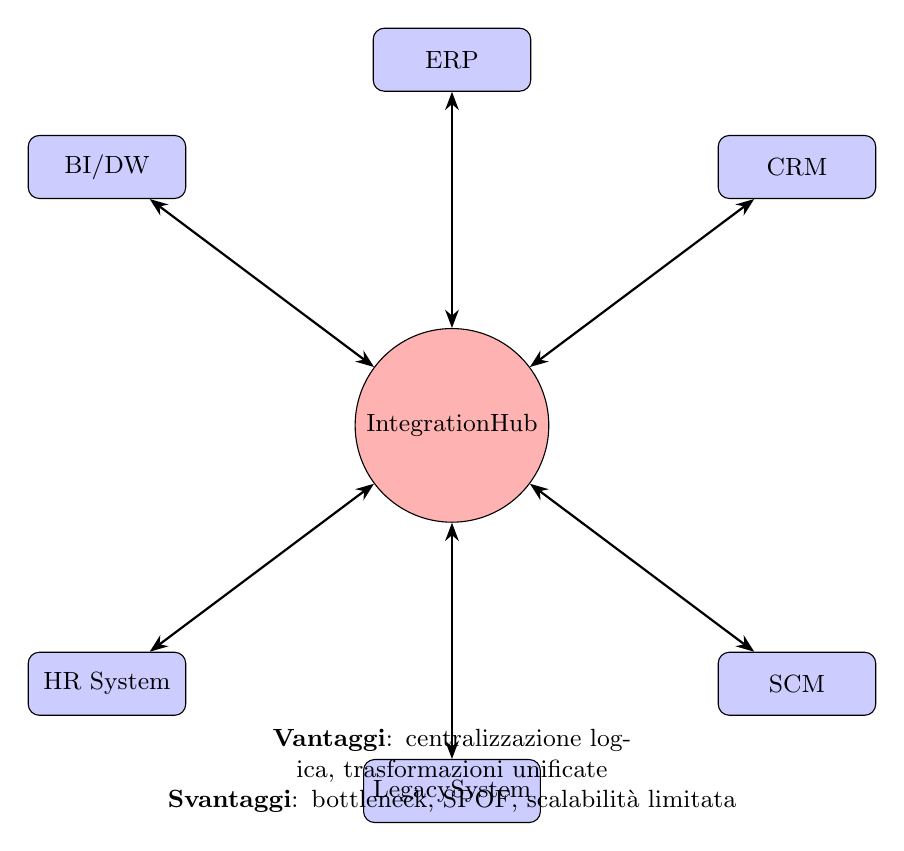
\begin{tikzpicture}[
				node distance=3cm,
				app/.style={draw,rectangle,rounded corners,minimum width=2cm,minimum height=0.8cm,fill=blue!20,font=\small},
				hub/.style={draw,circle,minimum size=2cm,fill=red!30,font=\small}
				]
				
				% Hub centrale
				\node[hub] (hub) {Integration\\Hub};
				
				% Applicazioni
				\node[app,above=of hub] (erp) {ERP};
				\node[app,above right=2cm and 2.5cm of hub] (crm) {CRM};
				\node[app,below right=2cm and 2.5cm of hub] (scm) {SCM};
				\node[app,below=of hub] (legacy) {Legacy\\System};
				\node[app,below left=2cm and 2.5cm of hub] (hr) {HR System};
				\node[app,above left=2cm and 2.5cm of hub] (bi) {BI/DW};
				
				% Connessioni bidirezionali
				\draw[{Stealth}-{Stealth},thick] (hub) -- (erp);
				\draw[{Stealth}-{Stealth},thick] (hub) -- (crm);
				\draw[{Stealth}-{Stealth},thick] (hub) -- (scm);
				\draw[{Stealth}-{Stealth},thick] (hub) -- (legacy);
				\draw[{Stealth}-{Stealth},thick] (hub) -- (hr);
				\draw[{Stealth}-{Stealth},thick] (hub) -- (bi);
				
				% Annotazione
				\node[below=2.5cm of hub,font=\small,text width=8cm,align=center] {
					\textbf{Vantaggi}: centralizzazione logica, trasformazioni unificate\\
					\textbf{Svantaggi}: bottleneck, SPOF, scalabilità limitata
				};
				
			\end{tikzpicture}
		\end{center}
	\end{frame}
	
	% 37
	\begin{frame}{Bus di integrazione}
		\textbf{Message Bus Architecture}
		
		\begin{block}{Concetto}
			Infrastruttura di comunicazione distribuita (bus logico) a cui tutte le applicazioni si connettono. Il bus gestisce routing, trasformazione e delivery dei messaggi.
		\end{block}
		
		\textbf{Vantaggi rispetto a Hub-and-Spoke:}
		\begin{itemize}
			\item \textbf{Scalabilità}: aggiunta nodi bus senza colli di bottiglia
			\item \textbf{Resilienza}: nessun single point of failure
			\item \textbf{Distribuzione geografica}: nodi in datacenter diversi
			\item \textbf{Specializzazione}: nodi dedicati per task specifici
		\end{itemize}
		
		\textbf{Sfide:}
		\begin{itemize}
			\item Complessità configurazione distribuita
			\item Governance e monitoraggio multi-nodo
			\item Consistenza routing rules
			\item Debugging più complesso
		\end{itemize}
		
		\textbf{Tecnologie:}
		\begin{itemize}
			\item Message-Oriented Middleware (MOM): IBM MQ, RabbitMQ, ActiveMQ
			\item Enterprise Service Bus (ESB): integra MOM con logica di integrazione
		\end{itemize}
	\end{frame}
	
	\section{Enterprise Service Bus}
	
	% 38
	\begin{frame}{Enterprise Service Bus: definizione}
		\textbf{ESB - Enterprise Service Bus}
		
		\begin{block}{Definizione formale}
			Architettura middleware che implementa un bus di comunicazione per integrare servizi eterogenei tramite routing intelligente, trasformazione dati, orchestrazione e gestione centralizzata delle policy.
		\end{block}
		
		\textbf{Funzionalità core:}
		\begin{itemize}
			\item \textbf{Routing}: intelligente, content-based, dinamico
			\item \textbf{Trasformazione}: XSLT, mapping, enrichment
			\item \textbf{Protocol mediation}: SOAP, REST, JMS, FTP, etc.
			\item \textbf{Service orchestration}: BPEL, flow control
			\item \textbf{Security}: autenticazione, autorizzazione, encryption
			\item \textbf{Transaction management}: distributed transactions
			\item \textbf{Monitoring & Management}: metriche, logging, audit
		\end{itemize}
		
		\textbf{Principi architetturali:}
		\begin{itemize}
			\item Loose coupling tra servizi
			\item Location transparency
			\item Protocol independence
			\item Mediation e adattamento
		\end{itemize}
	\end{frame}
	
	% 39
	\begin{frame}{Caratteristiche principali di ESB}
		\begin{columns}
			\column{0.48\textwidth}
			\textbf{Uniformità di accesso}
			\begin{itemize}
				\item Interfaccia uniforme verso il bus
				\item Nasconde eterogeneità sottostante
				\item Adattatori per legacy systems
			\end{itemize}
			
			\textbf{Disaccoppiamento}
			\begin{itemize}
				\item Servizi non si conoscono direttamente
				\item Comunicazione via bus
				\item Cambiamenti isolati
			\end{itemize}
			
			\textbf{Monitoring e QoS}
			\begin{itemize}
				\item SLA enforcement
				\item Metriche real-time
				\item Alert e notifiche
			\end{itemize}
			
			\column{0.48\textwidth}
			\textbf{Gestione centralizzata}
			\begin{itemize}
				\item Policy management
				\item Security governance
				\item Version control
			\end{itemize}
			
			\textbf{Scalabilità}
			\begin{itemize}
				\item Clustering e load balancing
				\item Horizontal scaling
				\item Failover automatico
			\end{itemize}
			
			\textbf{Logging e Audit}
			\begin{itemize}
				\item Message logging completo
				\item Tracciamento end-to-end
				\item Compliance e audit trail
			\end{itemize}
		\end{columns}
		
		\vspace{0.5cm}
		\begin{alertblock}{Nota}
			L'ESB non è solo tecnologia ma anche un pattern architetturale che guida la progettazione di sistemi integrati.
		\end{alertblock}
	\end{frame}
	
	% 40
	\begin{frame}{Schema: architettura ESB}
		\begin{center}
			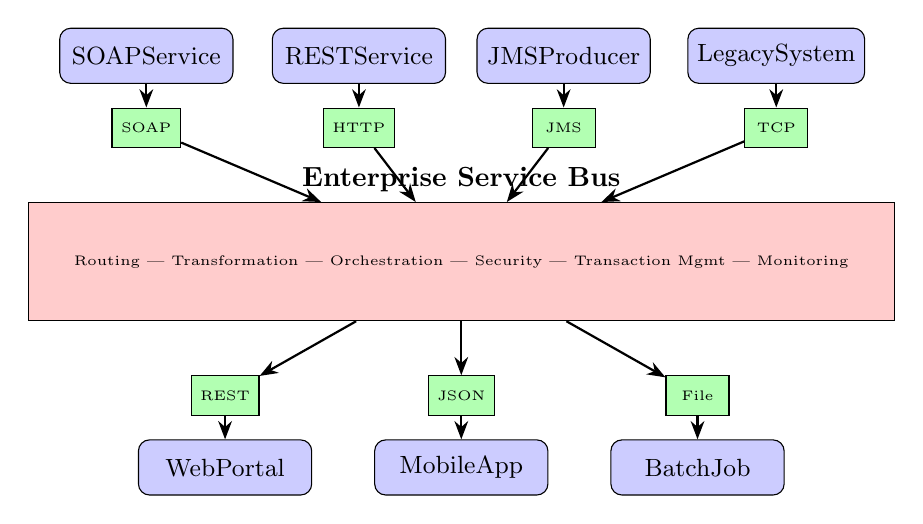
\begin{tikzpicture}[
				node distance=1.5cm,
				service/.style={draw,rectangle,rounded corners,minimum width=2.2cm,minimum height=0.7cm,fill=blue!20,font=\small},
				adapter/.style={draw,rectangle,minimum width=0.8cm,minimum height=0.5cm,fill=green!30,font=\tiny}
				]
				
				% ESB Bus centrale (ampio)
				\node[draw,rectangle,fill=red!20,minimum width=11cm,minimum height=1.5cm] (esb) {};
				\node[above] at (esb.north) {\textbf{Enterprise Service Bus}};
				\node[font=\tiny,text width=10cm,align=center] at (esb.center) {
					Routing | Transformation | Orchestration | Security | Transaction Mgmt | Monitoring
				};
				
				% Servizi sopra
				\node[service,above=of esb,xshift=-4cm] (soap) {SOAP\\Service};
				\node[service,above=of esb,xshift=-1.3cm] (rest) {REST\\Service};
				\node[service,above=of esb,xshift=1.3cm] (jms) {JMS\\Producer};
				\node[service,above=of esb,xshift=4cm] (legacy) {Legacy\\System};
				
				% Adattatori sopra
				\node[adapter,below=0.3cm of soap] (a1) {SOAP};
				\node[adapter,below=0.3cm of rest] (a2) {HTTP};
				\node[adapter,below=0.3cm of jms] (a3) {JMS};
				\node[adapter,below=0.3cm of legacy] (a4) {TCP};
				
				% Client/Portal sotto
				\node[service,below=of esb,xshift=-3cm] (web) {Web\\Portal};
				\node[service,below=of esb,xshift=0cm] (mobile) {Mobile\\App};
				\node[service,below=of esb,xshift=3cm] (batch) {Batch\\Job};
				
				% Adattatori sotto
				\node[adapter,above=0.3cm of web] (a5) {REST};
				\node[adapter,above=0.3cm of mobile] (a6) {JSON};
				\node[adapter,above=0.3cm of batch] (a7) {File};
				
				% Connessioni
				\draw[-{Stealth},thick] (soap) -- (a1);
				\draw[-{Stealth},thick] (a1) -- (esb);
				\draw[-{Stealth},thick] (rest) -- (a2);
				\draw[-{Stealth},thick] (a2) -- (esb);
				\draw[-{Stealth},thick] (jms) -- (a3);
				\draw[-{Stealth},thick] (a3) -- (esb);
				\draw[-{Stealth},thick] (legacy) -- (a4);
				\draw[-{Stealth},thick] (a4) -- (esb);
				
				\draw[-{Stealth},thick] (esb) -- (a5);
				\draw[-{Stealth},thick] (a5) -- (web);
				\draw[-{Stealth},thick] (esb) -- (a6);
				\draw[-{Stealth},thick] (a6) -- (mobile);
				\draw[-{Stealth},thick] (esb) -- (a7);
				\draw[-{Stealth},thick] (a7) -- (batch);
				
			\end{tikzpicture}
		\end{center}
	\end{frame}
	
	% 41
	\begin{frame}{Message Oriented Middleware}
		\textbf{MOM - Foundation dell'ESB}
		
		\begin{columns}
			\column{0.48\textwidth}
			\textbf{Queue (Point-to-Point)}
			\begin{itemize}
				\item Un producer, un consumer
				\item FIFO processing
				\item Load balancing tra consumer
				\item Garanzia di delivery
				\item Persistenza messaggi
			\end{itemize}
			
			\begin{center}
				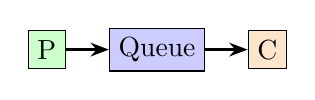
\begin{tikzpicture}[scale=0.7]
					\node[draw,rectangle,fill=green!20] (p) at (0,0) {P};
					\node[draw,rectangle,fill=blue!20] (q) at (2,0) {Queue};
					\node[draw,rectangle,fill=orange!20] (c) at (4,0) {C};
					\draw[-{Stealth},thick] (p) -- (q);
					\draw[-{Stealth},thick] (q) -- (c);
				\end{tikzpicture}
			\end{center}
			
			\column{0.48\textwidth}
			\textbf{Topic (Publish/Subscribe)}
			\begin{itemize}
				\item Un publisher, N subscriber
				\item Broadcasting
				\item Event-driven
				\item Durable/non-durable
				\item Message filtering
			\end{itemize}
			
			\begin{center}
				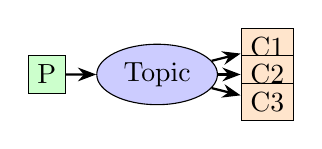
\begin{tikzpicture}[scale=0.7]
					\node[draw,rectangle,fill=green!20] (p) at (0,1) {P};
					\node[draw,ellipse,fill=blue!20] (t) at (2,1) {Topic};
					\node[draw,rectangle,fill=orange!20] (c1) at (4,1.5) {C1};
					\node[draw,rectangle,fill=orange!20] (c2) at (4,1) {C2};
					\node[draw,rectangle,fill=orange!20] (c3) at (4,0.5) {C3};
					\draw[-{Stealth},thick] (p) -- (t);
					\draw[-{Stealth},thick] (t) -- (c1);
					\draw[-{Stealth},thick] (t) -- (c2);
					\draw[-{Stealth},thick] (t) -- (c3);
				\end{tikzpicture}
			\end{center}
		\end{columns}
		
		\vspace{0.5cm}
		\textbf{Quality of Service (QoS):}
		\begin{itemize}
			\item \textbf{At-most-once}: possibile perdita messaggi
			\item \textbf{At-least-once}: possibili duplicati
			\item \textbf{Exactly-once}: delivery garantito una sola volta (costoso)
		\end{itemize}
	\end{frame}
	
	% 42
	\begin{frame}{Normalized Message Router (NMR)}
		\textbf{JBI Concept: Normalized Message Router}
		
		\begin{block}{Principio}
			I messaggi sono convertiti in un formato canonico neutro (normalized) all'ingresso nel bus. Le trasformazioni tra formati eterogenei avvengono solo ai bordi, non internamente.
		\end{block}
		
		\textbf{Vantaggi:}
		\begin{itemize}
			\item \textbf{Riduzione complessità}: O(n) adattatori invece di O(n²)
			\item \textbf{Riuso logica}: trasformazioni centralizzate
			\item \textbf{Loose coupling}: servizi non conoscono formati altrui
			\item \textbf{Manutenzione}: cambio formato esterno = 1 adattatore
		\end{itemize}
		
		\begin{center}
			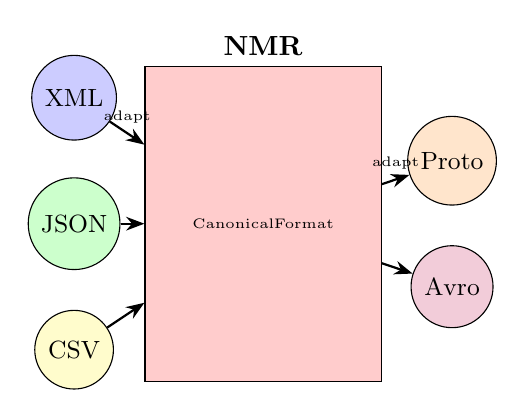
\begin{tikzpicture}[scale=0.8,node distance=1cm]
				% Formati esterni
				\node[draw,circle,fill=blue!20,font=\small] (xml) at (0,2) {XML};
				\node[draw,circle,fill=green!20,font=\small] (json) at (0,0) {JSON};
				\node[draw,circle,fill=yellow!20,font=\small] (csv) at (0,-2) {CSV};
				
				% NMR centrale
				\node[draw,rectangle,fill=red!20,minimum width=3cm,minimum height=4cm] (nmr) at (3,0) {};
				\node[above] at (nmr.north) {\textbf{NMR}};
				\node[font=\tiny] at (nmr.center) {Canonical\\Format};
				
				% Formati esterni destra
				\node[draw,circle,fill=orange!20,font=\small] (proto) at (6,1) {Proto};
				\node[draw,circle,fill=purple!20,font=\small] (avro) at (6,-1) {Avro};
				
				% Adattatori
				\draw[-{Stealth},thick] (xml) -- (nmr) node[midway,above,font=\tiny] {adapt};
				\draw[-{Stealth},thick] (json) -- (nmr);
				\draw[-{Stealth},thick] (csv) -- (nmr);
				\draw[-{Stealth},thick] (nmr) -- (proto) node[midway,above,font=\tiny] {adapt};
				\draw[-{Stealth},thick] (nmr) -- (avro);
				
			\end{tikzpicture}
		\end{center}
		
		\textbf{Canonical format tipico:} XML, JSON, o formato specifico del vendor ESB
	\end{frame}
	
	% 43
	\begin{frame}{JBI: Java Business Integration}
		\textbf{JSR 208 - Standard Java per ESB}
		
		\begin{block}{Obiettivo}
			Definire un'architettura standard e pluggable per integrare componenti di integrazione in Java. Permette interoperabilità tra vendor diversi.
		\end{block}
		
		\textbf{Componenti architetturali:}
		\begin{itemize}
			\item \textbf{Normalized Message Router (NMR)}: bus interno
			\item \textbf{Service Engine (SE)}: logica di business (BPEL, XSLT, validation)
			\item \textbf{Binding Component (BC)}: protocolli esterni (SOAP, HTTP, JMS, FTP)
			\item \textbf{JMX Management}: amministrazione e monitoraggio
		\end{itemize}
		
		\textbf{Normalized Message:}
		\begin{itemize}
			\item MessageExchange: contenitore dello scambio
			\item NormalizedMessage: payload + properties + attachments
			\item Pattern: In-Only, In-Out, etc.
		\end{itemize}
		
		\textbf{Implementazioni:}
		\begin{itemize}
			\item Apache ServiceMix
			\item OpenESB (GlassFish)
			\item PEtALS ESB
		\end{itemize}
		
		\textbf{Nota:} JBI oggi meno usato; sostituito da pattern più moderni (microservizi, service mesh)
	\end{frame}
	
	% 44
	\begin{frame}{Schema: JBI components}
		\begin{center}
			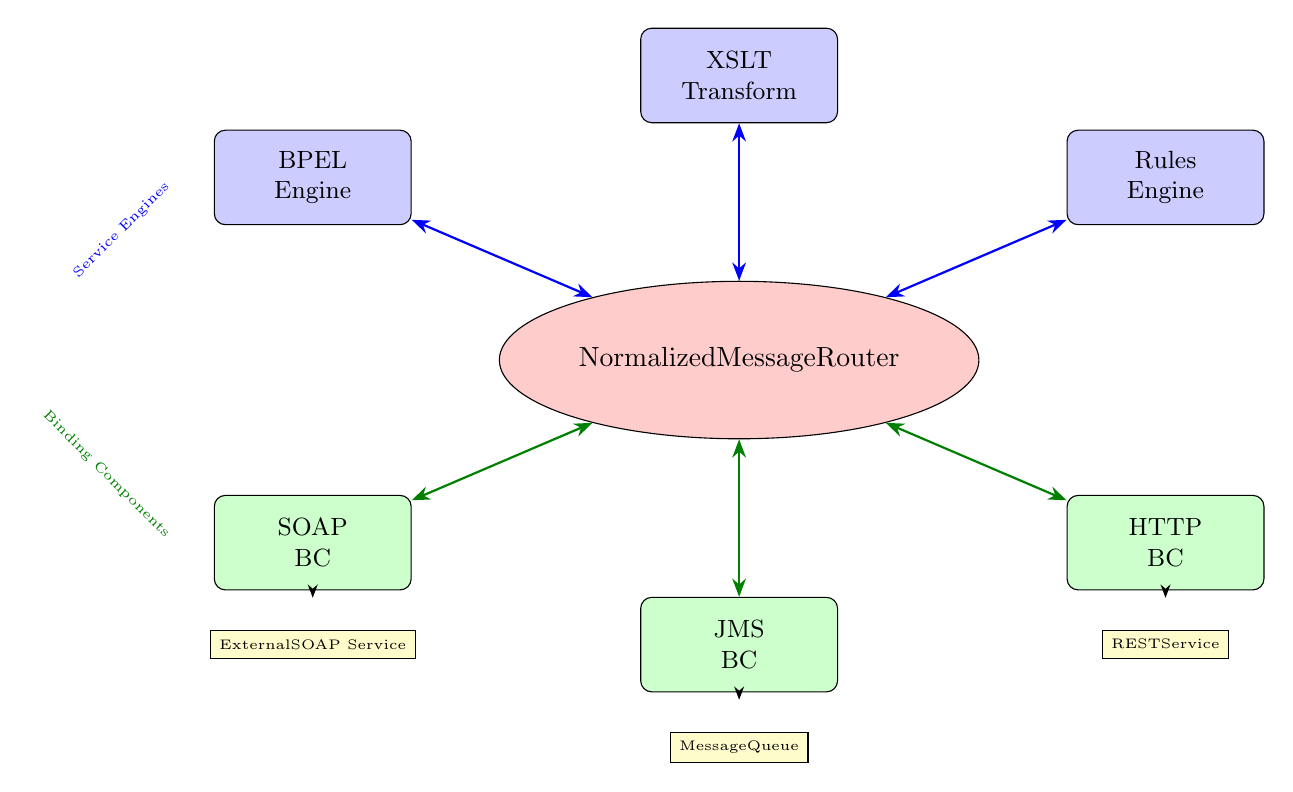
\begin{tikzpicture}[
				node distance=1.5cm,
				component/.style={draw,rectangle,rounded corners,minimum width=2.5cm,minimum height=1.2cm,font=\small,align=center},
				se/.style={component,fill=blue!20},
				bc/.style={component,fill=green!20}
				]
				
				% NMR centrale
				\node[draw,ellipse,fill=red!20,minimum width=4cm,minimum height=2cm] (nmr) {Normalized\\Message\\Router};
				
				% Service Engines (logica interna)
				\node[se,above left=1cm and 2cm of nmr] (bpel) {BPEL\\Engine};
				\node[se,above=2cm of nmr] (xslt) {XSLT\\Transform};
				\node[se,above right=1cm and 2cm of nmr] (rules) {Rules\\Engine};
				
				% Binding Components (protocolli esterni)
				\node[bc,below left=1cm and 2cm of nmr] (soap) {SOAP\\BC};
				\node[bc,below=2cm of nmr] (jms) {JMS\\BC};
				\node[bc,below right=1cm and 2cm of nmr] (http) {HTTP\\BC};
				
				% Connessioni SE <-> NMR
				\draw[{Stealth}-{Stealth},thick,blue] (bpel) -- (nmr);
				\draw[{Stealth}-{Stealth},thick,blue] (xslt) -- (nmr);
				\draw[{Stealth}-{Stealth},thick,blue] (rules) -- (nmr);
				
				% Connessioni BC <-> NMR
				\draw[{Stealth}-{Stealth},thick,green!50!black] (soap) -- (nmr);
				\draw[{Stealth}-{Stealth},thick,green!50!black] (jms) -- (nmr);
				\draw[{Stealth}-{Stealth},thick,green!50!black] (http) -- (nmr);
				
				% Etichette
				\node[left=0.5cm of bpel,rotate=45,font=\tiny,blue] {Service Engines};
				\node[left=0.5cm of soap,rotate=-45,font=\tiny,green!50!black] {Binding Components};
				
				% Sistemi esterni
				\node[draw,rectangle,fill=yellow!20,below=0.5cm of soap,font=\tiny] {External\\SOAP Service};
				\node[draw,rectangle,fill=yellow!20,below=0.5cm of jms,font=\tiny] {Message\\Queue};
				\node[draw,rectangle,fill=yellow!20,below=0.5cm of http,font=\tiny] {REST\\Service};
				
				\draw[-{Stealth}] (soap) -- ++(0,-0.7);
				\draw[-{Stealth}] (jms) -- ++(0,-0.7);
				\draw[-{Stealth}] (http) -- ++(0,-0.7);
				
			\end{tikzpicture}
		\end{center}
	\end{frame}
	
	% 45
	\begin{frame}{Pattern di scambio JBI}
		\textbf{Message Exchange Patterns (MEP)}
		
		\begin{table}
			\small
			\begin{tabular}{lp{7cm}}
				\textbf{Pattern} & \textbf{Descrizione} \\
				\hline
				\textbf{In-Only} & Fire-and-forget. Consumer invia messaggio senza aspettare risposta. Asincrono. \\
				\hline
				\textbf{Robust In-Only} & Come In-Only ma con acknowledgment o fault. \\
				\hline
				\textbf{In-Out} & Request-Response. Consumer invia e attende risposta. Sincrono o asincrono. \\
				\hline
				\textbf{In Optional-Out} & Consumer invia, risposta opzionale. Provider decide se rispondere. \\
				\hline
			\end{tabular}
		\end{table}
		
		\vspace{0.5cm}
		\textbf{Quando usarli:}
		\begin{itemize}
			\item \textbf{In-Only}: notifiche, logging, event broadcasting
			\item \textbf{Robust In-Only}: delivery garantito con ack
			\item \textbf{In-Out}: query, transazioni, richieste con risposta obbligatoria
			\item \textbf{In Optional-Out}: pattern flessibili, callback condizionali
		\end{itemize}
		
		\textbf{Gestione:}
		\begin{itemize}
			\item Il pattern è specificato dal consumer
			\item Il provider deve supportarlo o segnalare errore
			\item Il NMR gestisce il routing appropriato
		\end{itemize}
	\end{frame}
	
	% 46
	\begin{frame}{Routing e trasformazione}
		\textbf{Due pilastri dell'ESB}
		
		\begin{columns}
			\column{0.48\textwidth}
			\textbf{Routing}
			\begin{itemize}
				\item \textbf{Content-Based}: analisi payload
				\item \textbf{Header-Based}: metadata routing
				\item \textbf{Rule-Based}: business rules
				\item \textbf{Dynamic}: lookup runtime registry
			\end{itemize}
			
			\textbf{Esempio Content-Based:}
			\begin{itemize}
				\item Order amount < 1000 → Service A
				\item Order amount $\geq$ 1000 → Service B + approval
				\item Country = "IT" → Tax Service IT
			\end{itemize}
			
			\column{0.48\textwidth}
			\textbf{Trasformazione}
			\begin{itemize}
				\item \textbf{XSLT}: XML-to-XML
				\item \textbf{Data Mapper}: visual mapping
				\item \textbf{Custom Code}: Java, Groovy, etc.
				\item \textbf{Template}: Velocity, Freemarker
			\end{itemize}
			
			\textbf{Operazioni comuni:}
			\begin{itemize}
				\item Format conversion (XML$\leftrightarrow$JSON)
				\item Field mapping e renaming
				\item Data enrichment (lookup DB)
				\item Aggregation/splitting
				\item Validation e filtering
			\end{itemize}
		\end{columns}
		
		\vspace{0.5cm}
		\begin{block}{Best Practice}
			Trasformazioni complesse in Service Engine dedicati; routing in NMR. Separare logica di routing da logica di business.
		\end{block}
	\end{frame}
	
	% 47
	\begin{frame}{Pipeline di trasformazione: esempio}
		\textbf{Flusso end-to-end con trasformazioni multiple}
		
		\begin{center}
			\begin{tikzpicture}[
				node distance=1cm,
				step/.style={draw,rectangle,rounded corners,minimum width=2.3cm,minimum height=0.7cm,fill=blue!20,font=\footnotesize}
				]
				
				\node[step,fill=green!20] (input) {Input\\Message};
				\node[step,below=of input] (normalize) {1. Normalize};
				\node[step,below=of normalize] (validate) {2. Validate};
				\node[step,below=of validate] (enrich) {3. Enrich};
				\node[step,below=of enrich] (transform) {4. Transform};
				\node[step,below=of transform] (route) {5. Route};
				\node[step,below=of route] (delivery) {6. Delivery};
				\node[step,fill=orange!20,below=of delivery] (output) {Output\\Message};
				
				\draw[-{Stealth},thick] (input) -- (normalize) node[midway,right,font=\tiny,text width=2.5cm] {XML/JSON\\to Canonical};
				\draw[-{Stealth},thick] (normalize) -- (validate) node[midway,right,font=\tiny,text width=2.5cm] {XSD/Schema\\check};
				\draw[-{Stealth},thick] (validate) -- (enrich) node[midway,right,font=\tiny,text width=2.5cm] {DB lookup\\add metadata};
				\draw[-{Stealth},thick] (enrich) -- (transform) node[midway,right,font=\tiny,text width=2.5cm] {XSLT map\\to target};
				\draw[-{Stealth},thick] (transform) -- (route) node[midway,right,font=\tiny,text width=2.5cm] {Content-based\\routing};
				\draw[-{Stealth},thick] (route) -- (delivery) node[midway,right,font=\tiny,text width=2.5cm] {Protocol\\mediation};
				\draw[-{Stealth},thick] (delivery) -- (output);
				
				% Error handling laterale
				\node[draw,rectangle,fill=red!20,right=3cm of validate,font=\tiny,text width=1.5cm,align=center] (error) {Error\\Handler};
				\draw[-{Stealth},dashed,red] (validate) -- (error);
				\draw[-{Stealth},dashed,red] (enrich) -- (error);
				\draw[-{Stealth},dashed,red] (transform) -- (error);
				
			\end{tikzpicture}
		\end{center}
	\end{frame}
	
	% 48
	\begin{frame}{Monitoraggio e gestione operativa}
		\textbf{Observability nell'ESB}
		
		\textbf{Componenti chiave:}
		\begin{enumerate}
			\item \textbf{Logging}
			\begin{itemize}
				\item Message payload logging (attenzione dati sensibili!)
				\item Audit trail completo
				\item Correlation ID per tracking end-to-end
			\end{itemize}
			
			\item \textbf{Metrics}
			\begin{itemize}
				\item Throughput (msg/sec)
				\item Latency (percentili: p50, p95, p99)
				\item Error rate
				\item Queue depth
			\end{itemize}
			
			\item \textbf{Tracing Distribuito}
			\begin{itemize}
				\item Span per ogni hop
				\item Visualizzazione dependencies
				\item Bottleneck identification
			\end{itemize}
			
			\item \textbf{Alerting}
			\begin{itemize}
				\item Threshold-based alerts
				\item Anomaly detection
				\item Incident management integration
			\end{itemize}
		\end{enumerate}
		
		\textbf{Tool comuni:} ELK Stack, Prometheus/Grafana, Splunk, Dynatrace
	\end{frame}
	
	% 49
	\begin{frame}{Scalabilità e resilienza}
		\textbf{Tecniche per sistemi mission-critical}
		
		\begin{columns}
			\column{0.48\textwidth}
			\textbf{Scalabilità}
			\begin{itemize}
				\item \textbf{Clustering}: nodi ESB multipli
				\item \textbf{Load balancing}: distribuire carico
				\item \textbf{Sharding}: partizionamento dati
				\item \textbf{Caching}: ridurre latenza
				\item \textbf{Async processing}: decoupling temporale
			\end{itemize}
			
			\textbf{Horizontal Scaling:}
			\begin{itemize}
				\item Aggiungere nodi ESB
				\item Shared-nothing architecture
				\item Message queue distribuite
			\end{itemize}
			
			\column{0.48\textwidth}
			\textbf{Resilienza}
			\begin{itemize}
				\item \textbf{Failover}: switch automatico
				\item \textbf{Circuit breaker}: prevent cascading
				\item \textbf{Retry}: exponential backoff
				\item \textbf{Timeout}: limits attesa
				\item \textbf{Bulkhead}: isolamento failure
			\end{itemize}
			
			\textbf{High Availability:}
			\begin{itemize}
				\item Active-Active deployment
				\item Geographic redundancy
				\item Health checks continui
			\end{itemize}
		\end{columns}
		
		\vspace{0.5cm}
		\textbf{Back-pressure e Rate Limiting:}
		\begin{itemize}
			\item Protezione da overload
			\item Throttling consumer troppo veloci
			\item Queue sizing appropriato
		\end{itemize}
	\end{frame}
	
	% 50
	\begin{frame}{SLA e QoS}
		\textbf{Service Level Agreements e Quality of Service}
		
		\begin{block}{SLA - Service Level Agreement}
			Contratto tra provider e consumer che specifica metriche di performance, disponibilità e supporto. Spesso con penali per mancato rispetto.
		\end{block}
		
		\textbf{Metriche SLA tipiche:}
		\begin{itemize}
			\item \textbf{Availability}: 99.9\% uptime (43 min downtime/mese)
			\item \textbf{Response Time}: p95 < 200ms, p99 < 500ms
			\item \textbf{Throughput}: min 1000 req/sec
			\item \textbf{Error Rate}: < 0.1\%
			\item \textbf{MTTR}: Mean Time To Recovery < 15 min
		\end{itemize}
		
		\textbf{QoS nell'ESB:}
		\begin{itemize}
			\item \textbf{Priority queues}: messaggi critici prima
			\item \textbf{Resource reservation}: capacity dedicata
			\item \textbf{Rate limiting}: garantire fair usage
			\item \textbf{Circuit breaking}: protezione cascading failures
		\end{itemize}
		
		\textbf{Enforcement:}
		\begin{itemize}
			\item Monitoring continuo SLA compliance
			\item Alert quando threshold violati
			\item Reporting periodico ai stakeholder
		\end{itemize}
	\end{frame}
	
	\section{Casi d'Uso e Best Practices}
	
	% 51
	\begin{frame}{Esempio pratico: integrazione CRM-ERP}
		\textbf{Scenario: sincronizzazione ordini}
		
		\textbf{Requisito:}
		Quando un ordine viene creato nel CRM, deve essere automaticamente propagato all'ERP per la gestione magazzino e fatturazione.
		
		\textbf{Sequenza operazioni:}
		\begin{enumerate}
			\item \textbf{Trigger}: evento "NewOrder" dal CRM (via webhook o JMS)
			\item \textbf{ESB Reception}: Binding Component riceve evento
			\item \textbf{Normalizzazione}: conversione formato CRM → formato canonico
			\item \textbf{Validazione}: verifica completezza dati ordine
			\item \textbf{Enrichment}: lookup cliente in DB per dati fiscali
			\item \textbf{Trasformazione}: mapping formato canonico → formato ERP
			\item \textbf{Invocazione ERP}: chiamata SOAP/REST a ERP service
			\item \textbf{Gestione risposta}: 
			\begin{itemize}
				\item Successo: conferma a CRM
				\item Fallimento: retry logic o notifica manuale
			\end{itemize}
			\item \textbf{Audit}: logging completo transazione per compliance
		\end{enumerate}
		
		\textbf{Pattern applicati:} Content-Based Routing, Data Enrichment, Protocol Mediation
	\end{frame}
	
	% 52
	\begin{frame}{Diagramma: integrazione CRM-ERP}
		\begin{center}
			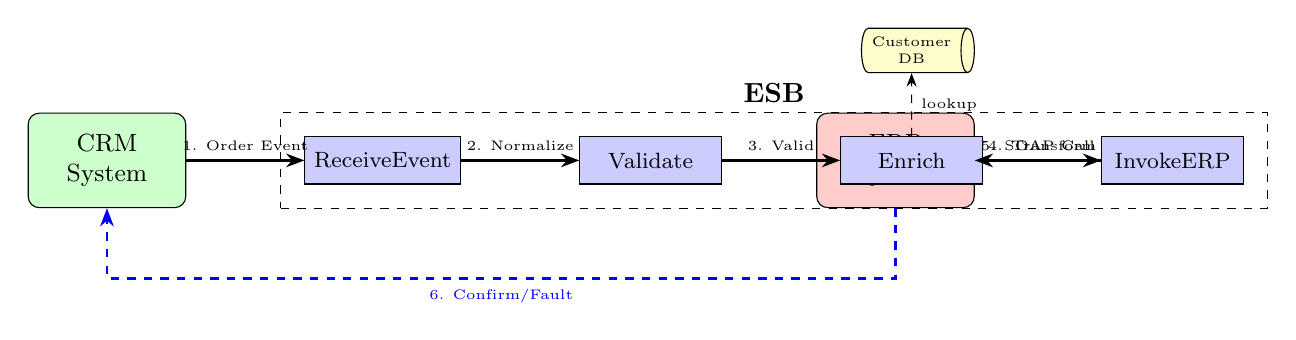
\begin{tikzpicture}[
				node distance=1.5cm,
				system/.style={draw,rectangle,rounded corners,minimum width=2cm,minimum height=1.2cm,font=\small,align=center},
				process/.style={draw,rectangle,minimum width=1.8cm,minimum height=0.6cm,fill=blue!20,font=\footnotesize}
				]
				
				% Sistemi
				\node[system,fill=green!20] (crm) {CRM\\System};
				\node[system,fill=red!20,right=8cm of crm] (erp) {ERP\\System};
				
				% ESB e processi
				\node[process,right=1.5cm of crm] (receive) {Receive\\Event};
				\node[process,right=of receive] (validate) {Validate};
				\node[process,right=of validate] (enrich) {Enrich};
				\node[process,right=of enrich] (invoke) {Invoke\\ERP};
				
				% Database per enrichment
				\node[draw,cylinder,shape aspect=0.3,fill=yellow!20,above=0.8cm of enrich,font=\tiny,align=center] (db) {Customer\\DB};
				
				% Frecce principali
				\draw[-{Stealth},thick] (crm) -- (receive) node[midway,above,font=\tiny] {1. Order Event};
				\draw[-{Stealth},thick] (receive) -- (validate) node[midway,above,font=\tiny] {2. Normalize};
				\draw[-{Stealth},thick] (validate) -- (enrich) node[midway,above,font=\tiny] {3. Valid};
				\draw[-{Stealth},thick] (enrich) -- (invoke) node[midway,above,font=\tiny] {4. Transform};
				\draw[-{Stealth},thick] (invoke) -- (erp) node[midway,above,font=\tiny] {5. SOAP Call};
				
				% Enrichment lookup
				\draw[-{Stealth},dashed] (enrich) -- (db) node[midway,right,font=\tiny] {lookup};
				
				% Risposta
				\draw[-{Stealth},thick,dashed,blue] (erp) -- ++(0,-1.5) -| (crm) node[near start,below,font=\tiny] {6. Confirm/Fault};
				
				% Box ESB
				\node[draw,rectangle,dashed,fit=(receive)(validate)(enrich)(invoke),inner sep=0.3cm,label=above:\textbf{ESB}] {};
				
			\end{tikzpicture}
		\end{center}
	\end{frame}
	
	% 53
	\begin{frame}{Rollback e compensazioni}
		\textbf{Compensating Transactions Pattern}
		
		\begin{block}{Problema}
			In sistemi distribuiti non è possibile usare transazioni ACID classiche. Servizi esterni potrebbero non supportare 2-phase commit.
		\end{block}
		
		\textbf{Soluzione: Saga Pattern}
		\begin{itemize}
			\item Sequenza di transazioni locali
			\item Ogni transazione ha una compensazione
			\item In caso di errore, esegui compensazioni in ordine inverso
		\end{itemize}
		
		\textbf{Esempio: prenotazione viaggio}
		\begin{enumerate}
			\item Prenota volo → Compensazione: cancella volo
			\item Prenota hotel → Compensazione: cancella hotel
			\item Prenota auto → Compensazione: cancella auto
			\item Errore al passo 3 → esegui: cancella hotel, cancella volo
		\end{enumerate}
		
		\textbf{Considerazioni:}
		\begin{itemize}
			\item Le compensazioni potrebbero fallire (gestire idempotenza)
			\item Eventual consistency invece di strong consistency
			\item Logging completo per audit e troubleshooting
			\item Possibili inconsistenze temporanee
		\end{itemize}
	\end{frame}
	
	% 54
	\begin{frame}{Testing di Web Services}
		\textbf{Strategie di test multi-livello}
		
		\begin{enumerate}
			\item \textbf{Unit Testing}
			\begin{itemize}
				\item Test singoli componenti in isolamento
				\item Mock di dipendenze esterne
				\item Framework: JUnit, TestNG, pytest
			\end{itemize}
			
			\item \textbf{Contract Testing}
			\begin{itemize}
				\item Validazione WSDL/schema
				\item Verifica input/output contract
				\item Tools: Pact, Spring Cloud Contract
			\end{itemize}
			
			\item \textbf{Integration Testing}
			\begin{itemize}
				\item Test flussi end-to-end
				\item Ambienti staging con servizi reali o stubs
				\item Tools: SoapUI, Postman, REST Assured
			\end{itemize}
			
			\item \textbf{Performance Testing}
			\begin{itemize}
				\item Load testing: throughput sotto carico
				\item Stress testing: comportamento al limite
				\item Tools: JMeter, Gatling, k6
			\end{itemize}
			
			\item \textbf{Security Testing}
			\begin{itemize}
				\item Penetration testing
				\item Vulnerability scanning
				\item Tools: OWASP ZAP, Burp Suite
			\end{itemize}
		\end{enumerate}
	\end{frame}
	
	% 55
	\begin{frame}{DevOps e CI/CD per servizi}
		\textbf{Pipeline automatizzata per Web Services}
		
		\textbf{Fasi della pipeline:}
		\begin{enumerate}
			\item \textbf{Source Control}
			\begin{itemize}
				\item Git repository per WSDL, XSD, code
				\item Branching strategy (GitFlow, trunk-based)
			\end{itemize}
			
			\item \textbf{Build}
			\begin{itemize}
				\item Compilazione codice
				\item Generazione artefatti (WAR, JAR)
				\item Validazione WSDL/XSD
			\end{itemize}
			
			\item \textbf{Test Automatici}
			\begin{itemize}
				\item Unit test, integration test
				\item Contract verification
				\item Code coverage report
			\end{itemize}
			
			\item \textbf{Deploy}
			\begin{itemize}
				\item Deploy su ambiente di staging
				\item Smoke tests
				\item Blue-green o canary deployment
			\end{itemize}
			
			\item \textbf{Monitoring}
			\begin{itemize}
				\item Health checks post-deploy
				\item Metriche real-time
				\item Alert configurati
			\end{itemize}
		\end{enumerate}
		
		\textbf{Tools:} Jenkins, GitLab CI, Azure DevOps, ArgoCD
	\end{frame}
	
	% 56
	\begin{frame}{Migration strategy}
		\textbf{Approccio incrementale legacy → ESB/SOA}
		
		\textbf{Fase 1: Assessment}
		\begin{itemize}
			\item Inventario sistemi esistenti
			\item Identificazione integrazioni point-to-point
			\item Analisi volumi e criticità
		\end{itemize}
		
		\textbf{Fase 2: Pilot}
		\begin{itemize}
			\item Selezione caso d'uso non critico
			\item Implementazione ESB per integrazione pilota
			\item Validazione approccio e ROI
		\end{itemize}
		
		\textbf{Fase 3: Expansion}
		\begin{itemize}
			\item Migrazione progressiva integrazioni
			\item Priorità su high-value / high-pain
			\item Approccio strangler fig pattern
		\end{itemize}
		
		\textbf{Fase 4: Consolidation}
		\begin{itemize}
			\item Dismissione integrazioni legacy
			\item Standardizzazione su ESB
			\item Governance e best practices
		\end{itemize}
		
		\textbf{Principi chiave:}
		\begin{itemize}
			\item Non big-bang: incrementale e reversibile
			\item Coesistenza legacy/nuovo durante transizione
			\item Training e change management
		\end{itemize}
	\end{frame}
	
	% 57
	\begin{frame}{Esempi di prodotti ESB}
		\textbf{Vendor e soluzioni open-source}
		
		\begin{table}
			\footnotesize
			\begin{tabular}{lll}
				\textbf{Prodotto} & \textbf{Tipo} & \textbf{Caratteristiche} \\
				\hline
				\textbf{Mule ESB} & Commercial & Potente, CloudHub, vasto ecosistema \\
				\textbf{WSO2 ESB} & Open Source & API-centric, microservices-ready \\
				\textbf{IBM Integration Bus} & Commercial & Enterprise-grade, mainframe integration \\
				\textbf{Apache ServiceMix} & Open Source & JBI-compliant, Karaf-based \\
				\textbf{Apache Camel} & Open Source & Routing engine, 300+ connectors \\
				\textbf{Red Hat Fuse} & Commercial & Basato su Camel, Kubernetes-native \\
				\textbf{Oracle SOA Suite} & Commercial & Full stack SOA, BPEL engine \\
				\textbf{Talend ESB} & Open Source & Data integration focus \\
			\end{tabular}
		\end{table}
		
		\vspace{0.3cm}
		\textbf{Trend attuali:}
		\begin{itemize}
			\item Shift verso API management e microservices
			\item Cloud-native ESB (service mesh, Istio, Linkerd)
			\item iPaaS (Integration Platform as a Service)
			\item Event-driven architecture (Kafka, event streaming)
		\end{itemize}
	\end{frame}
	
	% 58
	\begin{frame}{Confronto: Hub-and-Spoke vs Bus}
		\textbf{Sintesi dei trade-off}
		
		\begin{table}
			\small
			\begin{tabular}{|l|c|c|}
				\hline
				\textbf{Caratteristica} & \textbf{Hub-and-Spoke} & \textbf{Bus (ESB)} \\
				\hline
				\textbf{Scalabilità} & Limitata & Elevata \\
				\hline
				\textbf{SPOF Risk} & Alto & Basso \\
				\hline
				\textbf{Gestione} & Centralizzata (più semplice) & Distribuita (più complessa) \\
				\hline
				\textbf{Performance} & Bottleneck centrale & Distribuita \\
				\hline
				\textbf{Costo iniziale} & Basso & Medio-Alto \\
				\hline
				\textbf{Complessità} & Bassa & Media-Alta \\
				\hline
				\textbf{Manutenzione} & Più semplice & Più articolata \\
				\hline
				\textbf{Resilienza} & Bassa & Alta \\
				\hline
				\textbf{Geo-distribution} & Difficile & Nativa \\
				\hline
			\end{tabular}
		\end{table}
		
		\vspace{0.3cm}
		\textbf{Raccomandazione:}
		\begin{itemize}
			\item \textbf{Hub}: piccole-medie aziende, integrazioni limitate
			\item \textbf{ESB}: enterprise, high-volume, mission-critical
			\item \textbf{Ibrido}: hub + bus per bilanciare complessità e scalabilità
		\end{itemize}
	\end{frame}
	
	% 59
	\begin{frame}{Sicurezza nell'ESB}
		\textbf{Gestione centralizzata delle policy di sicurezza}
		
		\textbf{Vantaggi centralizzazione:}
		\begin{itemize}
			\item Policy security uniformi applicate a tutti i servizi
			\item Single point of enforcement
			\item Audit centralizzato
			\item Gestione certificati e credenziali centralizzata
		\end{itemize}
		
		\textbf{Meccanismi:}
		\begin{enumerate}
			\item \textbf{Authentication}
			\begin{itemize}
				\item OAuth 2.0 / OpenID Connect
				\item SAML assertions
				\item Certificati X.509
				\item API keys
			\end{itemize}
			
			\item \textbf{Authorization}
			\begin{itemize}
				\item RBAC (Role-Based Access Control)
				\item ABAC (Attribute-Based Access Control)
				\item Policy enforcement points
			\end{itemize}
			
			\item \textbf{Encryption}
			\begin{itemize}
				\item TLS/SSL per transport
				\item Message-level encryption (WS-Security)
				\item Key management e rotation
			\end{itemize}
			
			\item \textbf{Auditing}
			\begin{itemize}
				\item Logging accessi e operazioni
				\item Compliance reporting (GDPR, PCI-DSS)
				\item Intrusion detection
			\end{itemize}
		\end{enumerate}
	\end{frame}
	
	% 60
	\begin{frame}{Best practices architetturali}
		\textbf{Principi guida per progettazione robusta}
		
		\begin{enumerate}
			\item \textbf{Design for Failure}
			\begin{itemize}
				\item Assume ogni componente può fallire
				\item Circuit breakers, timeouts, retries
				\item Graceful degradation
			\end{itemize}
			
			\item \textbf{Idempotenza}
			\begin{itemize}
				\item Operazioni ripetibili senza effetti collaterali
				\item Essenziale per retry logic
				\item Usa unique message IDs
			\end{itemize}
			
			\item \textbf{Versioning}
			\begin{itemize}
				\item Versioning esplicito API e servizi
				\item Backward compatibility quando possibile
				\item Deprecation policy chiara
			\end{itemize}
			
			\item \textbf{Contratti stabili}
			\begin{itemize}
				\item WSDL/OpenAPI come contratto
				\item Consumer-driven contracts
				\item Breaking changes con major version bump
			\end{itemize}
			
			\item \textbf{Loose Coupling}
			\begin{itemize}
				\item Servizi indipendenti
				\item Comunicazione asincrona quando possibile
				\item Event-driven architectures
			\end{itemize}
		\end{enumerate}
	\end{frame}
	
	% 61
	\begin{frame}{Versioning dei servizi}
		\textbf{Strategie per evoluzione senza breaking changes}
		
		\begin{columns}
			\column{0.48\textwidth}
			\textbf{1. URL Versioning}
			\begin{itemize}
				\item \texttt{/api/v1/orders}
				\item \texttt{/api/v2/orders}
				\item Pro: esplicito, semplice
				\item Contro: proliferazione endpoint
			\end{itemize}
			
			\textbf{2. Header Versioning}
			\begin{itemize}
				\item \texttt{Accept: application/vnd.api+json; version=2}
				\item Pro: URL stabili
				\item Contro: meno visibile
			\end{itemize}
			
			\textbf{3. Query Parameter}
			\begin{itemize}
				\item \texttt{/api/orders?version=2}
				\item Pro: flessibile
				\item Contro: meno RESTful
			\end{itemize}
			
			\column{0.48\textwidth}
			\textbf{4. Namespace WSDL}
			\begin{itemize}
				\item \texttt{xmlns:v1="http://...v1"}
				\item \texttt{xmlns:v2="http://...v2"}
				\item Pro: standard SOAP
				\item Contro: verboso
			\end{itemize}
			
			\textbf{Compatibility Guidelines:}
			\begin{itemize}
				\item \textbf{Additive changes}: OK senza breaking
				\begin{itemize}
					\item Nuovi parametri opzionali
					\item Nuovi endpoint
					\item Nuovi campi response
				\end{itemize}
				\item \textbf{Breaking changes}: richiedono nuova versione
				\begin{itemize}
					\item Rimozione campi
					\item Cambio tipo dati
					\item Cambio semantica
				\end{itemize}
			\end{itemize}
		\end{columns}
		
		\vspace{0.3cm}
		\textbf{Deprecation:} comunicare in anticipo, mantenere versioni vecchie per periodo transizione
	\end{frame}
	
	% 62
	\begin{frame}{Governance in SOA}
		\textbf{Gestione del ciclo di vita dei servizi}
		
		\begin{block}{SOA Governance}
			Insieme di policy, processi e strumenti per assicurare che i servizi siano progettati, implementati, usati e mantenuti in modo coerente con gli obiettivi aziendali.
		\end{block}
		
		\textbf{Componenti:}
		\begin{enumerate}
			\item \textbf{Service Registry}
			\begin{itemize}
				\item Catalogo centralizzato servizi
				\item Metadati: owner, SLA, dependencies
				\item Stato: dev, test, prod, deprecated
			\end{itemize}
			
			\item \textbf{Policy Management}
			\begin{itemize}
				\item Naming conventions
				\item Security standards
				\item Performance requirements
			\end{itemize}
			
			\item \textbf{Lifecycle Management}
			\begin{itemize}
				\item Design → Development → Test → Deploy → Operate → Retire
				\item Approval gates tra fasi
				\item Change management
			\end{itemize}
			
			\item \textbf{Organizational Roles}
			\begin{itemize}
				\item Service owners
				\item Architects
				\item Governance board
			\end{itemize}
		\end{enumerate}
	\end{frame}
	
	% 63
	\begin{frame}{Metriche e KPI}
		\textbf{Key Performance Indicators per ESB/SOA}
		
		\begin{table}
			\footnotesize
			\begin{tabular}{llp{4cm}}
				\textbf{Metrica} & \textbf{Target tipico} & \textbf{Uso} \\
				\hline
				\textbf{Latency (p50)} & < 100ms & Performance media \\
				\textbf{Latency (p95)} & < 200ms & Outliers gestibili \\
				\textbf{Latency (p99)} & < 500ms & Worst-case acceptable \\
				\textbf{Throughput} & > 1000 req/s & Capacità sistema \\
				\textbf{Error Rate} & < 0.1\% & Affidabilità \\
				\textbf{Availability} & > 99.9\% & Uptime \\
				\textbf{MTBF} & > 720h (30 giorni) & Mean Time Between Failures \\
				\textbf{MTTR} & < 15 min & Mean Time To Recovery \\
				\textbf{Queue Depth} & < 1000 msg & Backlog monitoring \\
				\textbf{CPU Usage} & < 70\% & Resource utilization \\
			\end{tabular}
		\end{table}
		
		\vspace{0.3cm}
		\textbf{Dashboard e Alerting:}
		\begin{itemize}
			\item Real-time dashboard per ops team
			\item Alert quando threshold violati
			\item Trend analysis per capacity planning
			\item SLA compliance reporting
		\end{itemize}
	\end{frame}
	
	% 64
	\begin{frame}{Caso di studio sintetico}
		\textbf{Azienda manifatturiera: integrazione supply chain}
		
		\textbf{Scenario:}
		Azienda con ERP, sistemi fornitori esterni, portale B2B, magazzino automatizzato. Necessità di orchestrare ordini, spedizioni, fatturazione.
		
		\textbf{Architettura proposta:}
		\begin{itemize}
			\item \textbf{ESB centrale}: Mule ESB on-premise
			\item \textbf{Connettori}:
			\begin{itemize}
				\item SAP ERP (IDoc, RFC)
				\item Fornitori (REST API, EDI, email)
				\item Warehouse (SOAP WS)
				\item Portal B2B (REST/JSON)
			\end{itemize}
			\item \textbf{Orchestrazione}: BPEL per processo ordine completo
			\item \textbf{Monitoraggio}: ELK stack + Grafana
			\item \textbf{Sicurezza}: mTLS, OAuth tokens, API gateway
		\end{itemize}
		
		\textbf{Benefici ottenuti:}
		\begin{itemize}
			\item Riduzione 70\% tempi integrazione nuovi fornitori
			\item Eliminazione errori manuali (data entry)
			\item Visibilità real-time su supply chain
			\item Scaling da 100 a 500 ordini/ora senza re-engineering
		\end{itemize}
	\end{frame}
	
	% 65
	\begin{frame}{Esempio: flow end-to-end}
		\textbf{Tracciamento completo transazione}
		
		\begin{enumerate}
			\item \textbf{Evento iniziale}: Cliente crea ordine su portale web
			\begin{itemize}
				\item Timestamp: 2024-12-08T10:15:30Z
				\item Correlation ID: ORD-2024-123456
			\end{itemize}
			
			\item \textbf{Ingresso ESB}: HTTP POST ricevuto
			\begin{itemize}
				\item Validazione JWT token
				\item Logging request
			\end{itemize}
			
			\item \textbf{Orchestrazione BPEL}:
			\begin{itemize}
				\item Verifica disponibilità magazzino (SOAP call)
				\item Calcolo prezzo con sconti (Service Engine)
				\item Creazione ordine in ERP (SAP RFC)
				\item Notifica fornitori (JMS message)
			\end{itemize}
			
			\item \textbf{Sistema Terzo}: Fornitore conferma disponibilità
			\begin{itemize}
				\item Callback asincrono via REST
			\end{itemize}
			
			\item \textbf{Risposta}: Conferma ordine a cliente
			\begin{itemize}
				\item HTTP 200 + Order ID
				\item Email notifica
			\end{itemize}
			
			\item \textbf{Audit}: Log completo in DB audit
			\begin{itemize}
				\item Compliance GDPR
				\item Retention 7 anni
			\end{itemize}
		\end{enumerate}
	\end{frame}
	
	% 66
	\begin{frame}{Grafico: confronto throughput vs payload}
		\begin{center}
			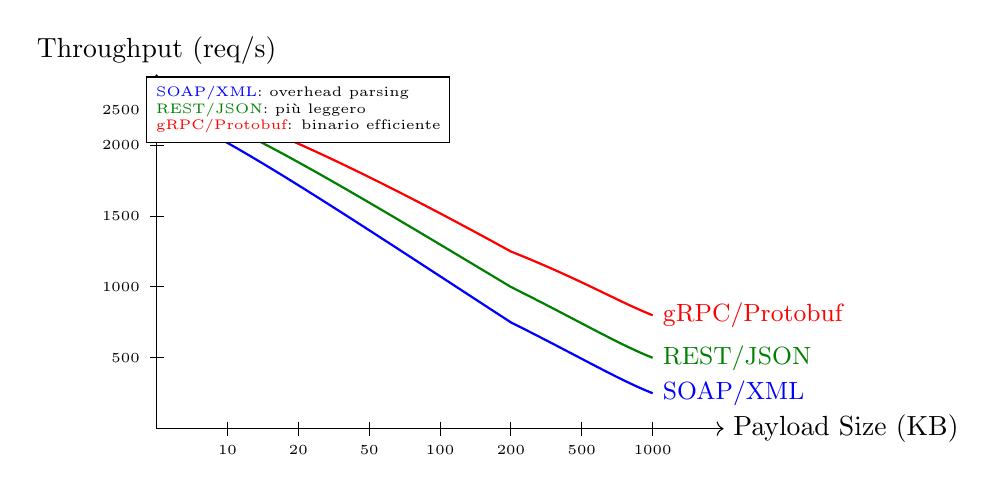
\begin{tikzpicture}[scale=0.9]
				
				% Assi
				\draw[->] (0,0) -- (8,0) node[right] {Payload Size (KB)};
				\draw[->] (0,0) -- (0,5) node[above] {Throughput (req/s)};
				
				% Ticks asse X
				\foreach \x/\label in {1/10,2/20,3/50,4/100,5/200,6/500,7/1000} {
					\draw (\x,0.1) -- (\x,-0.1) node[below,font=\tiny] {\label};
				}
				
				% Ticks asse Y
				\foreach \y/\label in {1/500,2/1000,3/1500,4/2000,4.5/2500} {
					\draw (0.1,\y) -- (-0.1,\y) node[left,font=\tiny] {\label};
				}
				
				% Curve
				\draw[thick,blue] (0.5,4.3) .. controls (1.5,3.8) and (3,2.8) .. (5,1.5) .. controls (6,1.0) and (6.5,0.7) .. (7,0.5) node[right,font=\small] {SOAP/XML};
				
				\draw[thick,green!50!black] (0.5,4.5) .. controls (1.5,4.1) and (3,3.2) .. (5,2.0) .. controls (6,1.5) and (6.5,1.2) .. (7,1.0) node[right,font=\small] {REST/JSON};
				
				\draw[thick,red] (0.5,4.6) .. controls (1.5,4.3) and (3,3.6) .. (5,2.5) .. controls (6,2.1) and (6.5,1.8) .. (7,1.6) node[right,font=\small] {gRPC/Protobuf};
				
				% Legenda
				\node[draw,rectangle,fill=white,align=left,font=\tiny] at (2,4.5) {
					\textcolor{blue}{SOAP/XML}: overhead parsing\\
					\textcolor{green!50!black}{REST/JSON}: più leggero\\
					\textcolor{red}{gRPC/Protobuf}: binario efficiente
				};
				
			\end{tikzpicture}
		\end{center}
		
		\textbf{Osservazioni:}
		\begin{itemize}
			\item Payload grandi penalizzano SOAP per overhead XML
			\item gRPC/Protobuf eccelle con dati strutturati complessi
			\item Per payload < 10KB le differenze sono minime
		\end{itemize}
	\end{frame}
	
	% 67
	\begin{frame}{Raccomandazioni progettuali}
		\textbf{Linee guida pratiche}
		
		\begin{enumerate}
			\item \textbf{Start Simple}
			\begin{itemize}
				\item Non over-engineer inizialmente
				\item Aggiungere complessità quando necessario
				\item Proof of concept prima di committare
			\end{itemize}
			
			\item \textbf{Document Everything}
			\begin{itemize}
				\item WSDL/OpenAPI sempre aggiornati
				\item Architettura diagrams
				\item Runbooks operativi
			\end{itemize}
			
			\item \textbf{Automate}
			\begin{itemize}
				\item CI/CD pipeline completa
				\item Infrastructure as Code
				\item Automated testing
			\end{itemize}
			
			\item \textbf{Monitor Proactively}
			\begin{itemize}
				\item Non aspettare problemi per monitorare
				\item Baseline metrics in produzione
				\item Capacity planning basato su trend
			\end{itemize}
			
			\item \textbf{Security by Design}
			\begin{itemize}
				\item Non aggiungere sicurezza dopo
				\item Threat modeling in fase design
				\item Regular security audits
			\end{itemize}
			
			\item \textbf{Plan for Evolution}
			\begin{itemize}
				\item Architettura deve supportare cambiamento
				\item Versioning strategy dall'inizio
				\item Evitare tight coupling
			\end{itemize}
		\end{enumerate}
	\end{frame}
	
	\section{Conclusioni}
	
	% 68
	\begin{frame}{Prospettive future}
		\textbf{Tendenze emergenti}
		
		\textbf{1. Shift verso architetture moderne:}
		\begin{itemize}
			\item \textbf{Microservizi}: granularità fine, deploy indipendenti
			\item \textbf{Service Mesh}: Istio, Linkerd per comunicazione service-to-service
			\item \textbf{Serverless}: FaaS per integrazione event-driven
		\end{itemize}
		
		\textbf{2. API-first design:}
		\begin{itemize}
			\item REST/JSON dominante per semplicità
			\item GraphQL per query flessibili
			\item gRPC per performance critical
			\item AsyncAPI per event-driven
		\end{itemize}
		
		\textbf{3. Cloud-native integration:}
		\begin{itemize}
			\item iPaaS (Integration Platform as a Service)
			\item Managed ESB in cloud (Azure Integration Services, AWS AppFlow)
			\item Kubernetes-native integration (Knative, Camel-K)
		\end{itemize}
		
		\textbf{4. Event streaming:}
		\begin{itemize}
			\item Apache Kafka per real-time data pipelines
			\item Event sourcing e CQRS patterns
			\item Stream processing (Kafka Streams, Flink)
		\end{itemize}
		
		\textbf{5. AI/ML integration:}
		\begin{itemize}
			\item Intelligent routing e transformation
			\item Anomaly detection automatico
			\item Predictive scaling
		\end{itemize}
	\end{frame}
	
	% 69
	\begin{frame}{Risorse e letture consigliate}
		\textbf{Standard e Specifiche:}
		\begin{itemize}
			\item W3C SOAP Specifications: \url{https://www.w3.org/TR/soap/}
			\item W3C WSDL 2.0: \url{https://www.w3.org/TR/wsdl20/}
			\item OASIS WS-* Specifications: \url{https://www.oasis-open.org/}
			\item JSR 208 JBI: \url{https://jcp.org/en/jsr/detail?id=208}
		\end{itemize}
		
		\textbf{Libri di riferimento:}
		\begin{itemize}
			\item "Enterprise Integration Patterns" - Hohpe \& Woolf
			\item "SOA Principles of Service Design" - Thomas Erl
			\item "Web Services Essentials" - Cerami
			\item "Building Microservices" - Sam Newman
		\end{itemize}
		
		\textbf{Progetti Open Source:}
		\begin{itemize}
			\item Apache Camel: \url{https://camel.apache.org/}
			\item Apache ServiceMix: \url{https://servicemix.apache.org/}
			\item WSO2: \url{https://wso2.com/}
			\item Mule (Community): \url{https://www.mulesoft.com/}
		\end{itemize}
		
		\textbf{Tutorial e Corsi:}
		\begin{itemize}
			\item Udemy, Coursera, Pluralsight: corsi su SOA, ESB, Web Services
			\item Red Hat Developer: hands-on labs
		\end{itemize}
	\end{frame}
	
	% 70
	\begin{frame}{Conclusioni}
		\textbf{Punti chiave della presentazione}
		
		\begin{enumerate}
			\item \textbf{Web Services} hanno rivoluzionato l'integrazione enterprise con standard aperti e firewall-friendly
			
			\item \textbf{SOAP/WSDL/UDDI} formano la base tecnica ma con complessità significativa
			
			\item \textbf{ESB} rappresenta l'evoluzione da integrazioni point-to-point a architetture scalabili e governate
			
			\item \textbf{Orchestrazione e coreografia} permettono composizione di processi complessi
			
			\item \textbf{Governance, monitoraggio, sicurezza} sono pilastri per deployment enterprise
			
			\item \textbf{Futuro} è verso microservizi, service mesh, API management e event streaming
		\end{enumerate}
		
		\vspace{0.5cm}
		\begin{block}{Suggerimenti per approfondire}
			\begin{itemize}
				\item Sperimentare con progetti open-source (Camel, ServiceMix)
				\item Studiare Enterprise Integration Patterns
				\item Progettare caso d'uso reale e implementare POC
				\item Seguire evoluzione verso architetture cloud-native
			\end{itemize}
		\end{block}
		
		\vspace{0.3cm}
		\centering
		\Large{\textbf{Domande?}}
	\end{frame}
	
\end{document}